\documentclass[twoside]{book}

% Packages required by doxygen
\usepackage{calc}
\usepackage{doxygen}
\usepackage{graphicx}
\usepackage[utf8]{inputenc}
\usepackage{makeidx}
\usepackage{multicol}
\usepackage{multirow}
\usepackage{textcomp}
\usepackage[table]{xcolor}

% Font selection
\usepackage[T1]{fontenc}
\usepackage{mathptmx}
\usepackage[scaled=.90]{helvet}
\usepackage{courier}
\usepackage{amssymb}
\usepackage{sectsty}
\renewcommand{\familydefault}{\sfdefault}
\allsectionsfont{%
  \fontseries{bc}\selectfont%
  \color{darkgray}%
}
\renewcommand{\DoxyLabelFont}{%
  \fontseries{bc}\selectfont%
  \color{darkgray}%
}

% Page & text layout
\usepackage{geometry}
\geometry{%
  a4paper,%
  top=2.5cm,%
  bottom=2.5cm,%
  left=2.5cm,%
  right=2.5cm%
}
\tolerance=750
\hfuzz=15pt
\hbadness=750
\setlength{\emergencystretch}{15pt}
\setlength{\parindent}{0cm}
\setlength{\parskip}{0.2cm}
\makeatletter
\renewcommand{\paragraph}{%
  \@startsection{paragraph}{4}{0ex}{-1.0ex}{1.0ex}{%
    \normalfont\normalsize\bfseries\SS@parafont%
  }%
}
\renewcommand{\subparagraph}{%
  \@startsection{subparagraph}{5}{0ex}{-1.0ex}{1.0ex}{%
    \normalfont\normalsize\bfseries\SS@subparafont%
  }%
}
\makeatother

% Headers & footers
\usepackage{fancyhdr}
\pagestyle{fancyplain}
\fancyhead[LE]{\fancyplain{}{\bfseries\thepage}}
\fancyhead[CE]{\fancyplain{}{}}
\fancyhead[RE]{\fancyplain{}{\bfseries\leftmark}}
\fancyhead[LO]{\fancyplain{}{\bfseries\rightmark}}
\fancyhead[CO]{\fancyplain{}{}}
\fancyhead[RO]{\fancyplain{}{\bfseries\thepage}}
\fancyfoot[LE]{\fancyplain{}{}}
\fancyfoot[CE]{\fancyplain{}{}}
\fancyfoot[RE]{\fancyplain{}{\bfseries\scriptsize Generated on Thu Sep 18 2014 15:19:30 for PivotApproach by Doxygen }}
\fancyfoot[LO]{\fancyplain{}{\bfseries\scriptsize Generated on Thu Sep 18 2014 15:19:30 for PivotApproach by Doxygen }}
\fancyfoot[CO]{\fancyplain{}{}}
\fancyfoot[RO]{\fancyplain{}{}}
\renewcommand{\footrulewidth}{0.4pt}
\renewcommand{\chaptermark}[1]{%
  \markboth{#1}{}%
}
\renewcommand{\sectionmark}[1]{%
  \markright{\thesection\ #1}%
}

% Indices & bibliography
\usepackage{natbib}
\usepackage[titles]{tocloft}
\setcounter{tocdepth}{3}
\setcounter{secnumdepth}{5}
\makeindex

% Hyperlinks (required, but should be loaded last)
\usepackage{ifpdf}
\ifpdf
  \usepackage[pdftex,pagebackref=true]{hyperref}
\else
  \usepackage[ps2pdf,pagebackref=true]{hyperref}
\fi
\hypersetup{%
  colorlinks=true,%
  linkcolor=blue,%
  citecolor=blue,%
  unicode%
}

% Custom commands
\newcommand{\clearemptydoublepage}{%
  \newpage{\pagestyle{empty}\cleardoublepage}%
}


%===== C O N T E N T S =====

\begin{document}

% Titlepage & ToC
\hypersetup{pageanchor=false}
\pagenumbering{roman}
\begin{titlepage}
\vspace*{7cm}
\begin{center}%
{\Large Pivot\-Approach \\[1ex]\large 001 }\\
\vspace*{1cm}
{\large Generated by Doxygen 1.8.3.1-20130402}\\
\vspace*{0.5cm}
{\small Thu Sep 18 2014 15:19:30}\\
\end{center}
\end{titlepage}
\clearemptydoublepage
\tableofcontents
\clearemptydoublepage
\pagenumbering{arabic}
\hypersetup{pageanchor=true}

%--- Begin generated contents ---
\chapter{Pivot\-Approach}
\label{md_README}
\hypertarget{md_README}{}
This repository codes related to the research performed by Dr. Juan Rojas. It implements snap assemblies using the Pivot\-Approach. 
\chapter{Todo List}
\label{todo}
\hypertarget{todo}{}

\begin{DoxyRefList}
\item[\label{todo__todo000003}%
\hypertarget{todo__todo000003}{}%
Member \hyperlink{classOpenHRP_1_1CFSImpl_a3032163447ca65ec81dc2a5c29cecf34}{Open\-H\-R\-P\-:\-:C\-F\-S\-Impl\-:\-:extract\-Rel\-Accels\-From\-Link\-Pair\-Case1} (matrix\-\_\-range$<$ rmdmatrix $>$ \&Kxn, matrix\-\_\-range$<$ rmdmatrix $>$ \&Kxt, Link\-Pair \&link\-Pair, int test\-Force\-Index, int constraint\-Index)]Can the follwoing equations be simplified ?  
\item[\label{todo__todo000001}%
\hypertarget{todo__todo000001}{}%
Member \hyperlink{classOpenHRP_1_1CFSImpl_aa85768ddd80a84f7ab6f038ef21e1869}{Open\-H\-R\-P\-:\-:C\-F\-S\-Impl\-:\-:set\-Acceleration\-Matrix} ()]This code does not work correctly when the links are in the same body. Fix it. 

This code does not work correctly when the links are in the same body. Fix it. 
\end{DoxyRefList}
\chapter{Hierarchical Index}
\section{Class Hierarchy}
This inheritance list is sorted roughly, but not completely, alphabetically\-:\begin{DoxyCompactList}
\item \contentsline{section}{Assembly\-Strategy}{\pageref{classAssemblyStrategy}}{}
\item \contentsline{section}{Open\-H\-R\-P\-:\-:C\-F\-S\-Impl\-:\-:Body\-Data}{\pageref{structOpenHRP_1_1CFSImpl_1_1BodyData}}{}
\item \contentsline{section}{Open\-H\-R\-P\-:\-:C\-F\-S\-Impl}{\pageref{classOpenHRP_1_1CFSImpl}}{}
\item \contentsline{section}{Open\-H\-R\-P\-:\-:C\-F\-S\-Impl\-:\-:Constraint\-Point}{\pageref{structOpenHRP_1_1CFSImpl_1_1ConstraintPoint}}{}
\item \contentsline{section}{Control\-Basis}{\pageref{classControlBasis}}{}
\item \contentsline{section}{Filter\-Tools}{\pageref{classFilterTools}}{}
\item \contentsline{section}{hiro\-Arm}{\pageref{classhiroArm}}{}
\begin{DoxyCompactList}
\item \contentsline{section}{hiro\-Arm\-Mas}{\pageref{classhiroArmMas}}{}
\item \contentsline{section}{hiro\-Arm\-Sla}{\pageref{classhiroArmSla}}{}
\end{DoxyCompactList}
\item \contentsline{section}{Open\-H\-R\-P\-:\-:C\-F\-S\-Impl\-:\-:Link\-Data}{\pageref{structOpenHRP_1_1CFSImpl_1_1LinkData}}{}
\item \contentsline{section}{Open\-H\-R\-P\-:\-:C\-F\-S\-Impl\-:\-:Link\-Pair}{\pageref{structOpenHRP_1_1CFSImpl_1_1LinkPair}}{}
\item \contentsline{section}{nitta\-F\-S}{\pageref{classnittaFS}}{}
\item \contentsline{section}{hiro\-Arm\-:\-:path\-\_\-params}{\pageref{structhiroArm_1_1path__params}}{}
\item plugin\begin{DoxyCompactList}
\item \contentsline{section}{force\-Sensor\-Plugin\-\_\-impl}{\pageref{classforceSensorPlugin__impl}}{}
\end{DoxyCompactList}
\item P\-O\-A\-\_\-force\-Sensor\-Plugin\begin{DoxyCompactList}
\item \contentsline{section}{force\-Sensor\-Plugin\-\_\-impl}{\pageref{classforceSensorPlugin__impl}}{}
\end{DoxyCompactList}
\item Ref\-Count\-Servant\-Base\begin{DoxyCompactList}
\item \contentsline{section}{force\-Sensor\-Plugin\-\_\-impl}{\pageref{classforceSensorPlugin__impl}}{}
\end{DoxyCompactList}
\end{DoxyCompactList}

\chapter{Class Index}
\section{Class List}
Here are the classes, structs, unions and interfaces with brief descriptions\-:\begin{DoxyCompactList}
\item\contentsline{section}{\hyperlink{classAssemblyStrategy}{Assembly\-Strategy} }{\pageref{classAssemblyStrategy}}{}
\item\contentsline{section}{\hyperlink{structOpenHRP_1_1CFSImpl_1_1BodyData}{Open\-H\-R\-P\-::\-C\-F\-S\-Impl\-::\-Body\-Data} }{\pageref{structOpenHRP_1_1CFSImpl_1_1BodyData}}{}
\item\contentsline{section}{\hyperlink{classOpenHRP_1_1CFSImpl}{Open\-H\-R\-P\-::\-C\-F\-S\-Impl} }{\pageref{classOpenHRP_1_1CFSImpl}}{}
\item\contentsline{section}{\hyperlink{structOpenHRP_1_1CFSImpl_1_1ConstraintPoint}{Open\-H\-R\-P\-::\-C\-F\-S\-Impl\-::\-Constraint\-Point} }{\pageref{structOpenHRP_1_1CFSImpl_1_1ConstraintPoint}}{}
\item\contentsline{section}{\hyperlink{classControlBasis}{Control\-Basis} }{\pageref{classControlBasis}}{}
\item\contentsline{section}{\hyperlink{classFilterTools}{Filter\-Tools} }{\pageref{classFilterTools}}{}
\item\contentsline{section}{\hyperlink{classforceSensorPlugin__impl}{force\-Sensor\-Plugin\-\_\-impl} }{\pageref{classforceSensorPlugin__impl}}{}
\item\contentsline{section}{\hyperlink{classhiroArm}{hiro\-Arm} }{\pageref{classhiroArm}}{}
\item\contentsline{section}{\hyperlink{classhiroArmMas}{hiro\-Arm\-Mas} }{\pageref{classhiroArmMas}}{}
\item\contentsline{section}{\hyperlink{classhiroArmSla}{hiro\-Arm\-Sla} }{\pageref{classhiroArmSla}}{}
\item\contentsline{section}{\hyperlink{structOpenHRP_1_1CFSImpl_1_1LinkData}{Open\-H\-R\-P\-::\-C\-F\-S\-Impl\-::\-Link\-Data} }{\pageref{structOpenHRP_1_1CFSImpl_1_1LinkData}}{}
\item\contentsline{section}{\hyperlink{structOpenHRP_1_1CFSImpl_1_1LinkPair}{Open\-H\-R\-P\-::\-C\-F\-S\-Impl\-::\-Link\-Pair} }{\pageref{structOpenHRP_1_1CFSImpl_1_1LinkPair}}{}
\item\contentsline{section}{\hyperlink{classnittaFS}{nitta\-F\-S} }{\pageref{classnittaFS}}{}
\item\contentsline{section}{\hyperlink{structhiroArm_1_1path__params}{hiro\-Arm\-::path\-\_\-params} }{\pageref{structhiroArm_1_1path__params}}{}
\end{DoxyCompactList}

\chapter{File Index}
\section{File List}
Here is a list of all documented files with brief descriptions\-:\begin{DoxyCompactList}
\item\contentsline{section}{{\bfseries Assembly\-Strategy.\-h} }{\pageref{AssemblyStrategy_8h}}{}
\item\contentsline{section}{\hyperlink{ConstraintForceSolver_8cpp}{Constraint\-Force\-Solver.\-cpp} \\*Implementation of Contact\-Force\-Solver class }{\pageref{ConstraintForceSolver_8cpp}}{}
\item\contentsline{section}{{\bfseries Control\-Basis.\-h} }{\pageref{ControlBasis_8h}}{}
\item\contentsline{section}{{\bfseries Filter\-Tools.\-h} }{\pageref{FilterTools_8h}}{}
\item\contentsline{section}{{\bfseries force\-Sensor\-Plugin\-\_\-impl.\-h} }{\pageref{forceSensorPlugin__impl_8h}}{}
\item\contentsline{section}{\hyperlink{hiroArm_8cpp}{hiro\-Arm.\-cpp} \\*Arm class for H\-I\-R\-O }{\pageref{hiroArm_8cpp}}{}
\item\contentsline{section}{\hyperlink{hiroArm_8h}{hiro\-Arm.\-h} \\*Arm class for H\-I\-R\-O }{\pageref{hiroArm_8h}}{}
\item\contentsline{section}{\hyperlink{nittaFS_8cpp}{nitta\-F\-S.\-cpp} \\*Nitta force moment sensor class }{\pageref{nittaFS_8cpp}}{}
\item\contentsline{section}{\hyperlink{nittaFS_8h}{nitta\-F\-S.\-h} \\*Nitta force moment sensor class }{\pageref{nittaFS_8h}}{}
\end{DoxyCompactList}

\chapter{Class Documentation}
\hypertarget{classAssemblyStrategy}{\section{Assembly\-Strategy Class Reference}
\label{classAssemblyStrategy}\index{Assembly\-Strategy@{Assembly\-Strategy}}
}
\subsection*{Public Types}
\begin{DoxyCompactItemize}
\item 
enum {\bfseries Control\-Paradigm} \{ {\bfseries motion\-Data}, 
{\bfseries control\-Basis}
 \}
\item 
enum {\bfseries Controller\-Type} \{ {\bfseries Null}, 
{\bfseries Position\-Ctrl}, 
{\bfseries Force\-Ctrl}, 
{\bfseries Moment\-Ctrl}
 \}
\item 
enum {\bfseries Ctrl\-Strategy} \{ {\bfseries Manipulation\-Test}, 
{\bfseries Straight\-Line\-Approach}, 
{\bfseries Pivot\-Approach}, 
{\bfseries Side\-Approach}
 \}
\item 
enum {\bfseries Test\-Axis} \{ \\*
{\bfseries pos\-Fx}, 
{\bfseries neg\-Fx}, 
{\bfseries pos\-Fy}, 
{\bfseries neg\-Fy}, 
\\*
{\bfseries pos\-Fz}, 
{\bfseries neg\-Fz}, 
{\bfseries pos\-Mx}, 
{\bfseries neg\-Mx}, 
\\*
{\bfseries pos\-My}, 
{\bfseries neg\-My}, 
{\bfseries pos\-Mz}, 
{\bfseries neg\-Mz}, 
\\*
{\bfseries all}, 
{\bfseries none}
 \}
\item 
enum {\bfseries ctrl\-Comp} \{ \\*
{\bfseries Position\-Composition} = 1, 
{\bfseries Position\-Orientation\-Composition}, 
{\bfseries Pose\-Composition}, 
{\bfseries I\-Kin\-Composition}, 
\\*
{\bfseries I\-Kin\-Force\-Composition}, 
{\bfseries I\-Kin\-Moment\-Composition}, 
{\bfseries Force\-Composition}, 
{\bfseries Force\-I\-Kin\-Composition}, 
\\*
{\bfseries Force\-Moment\-Composition}, 
{\bfseries F\-M\-P\-Composition}, 
{\bfseries Moment\-Composition}, 
{\bfseries Moment\-I\-Kin\-Composition}, 
\\*
{\bfseries Moment\-Force\-Composition}, 
{\bfseries Moment\-Force\-I\-Kin\-Composition}, 
{\bfseries M\-F\-P\-Composition}
 \}
\item 
enum {\bfseries force\-Axes} \{ \\*
{\bfseries Fx}, 
{\bfseries Fy}, 
{\bfseries Fz}, 
{\bfseries Mx}, 
\\*
{\bfseries My}, 
{\bfseries Mz}
 \}
\item 
enum {\bfseries P\-A10\-\_\-\-P\-A\-\_\-\-States} \{ \\*
{\bfseries pa\-Approach} = 1, 
{\bfseries pa\-Rotation}, 
{\bfseries pa\-Alignment}, 
{\bfseries pa\-Insertion}, 
\\*
{\bfseries pa\-Mating}, 
{\bfseries pa\-Finish}
 \}
\item 
enum {\bfseries H\-I\-R\-O\-\_\-\-S\-A\-\_\-\-States} \{ \\*
{\bfseries hsa\-Approach} = 1, 
{\bfseries hsa\-Rotation}, 
{\bfseries hsa\-Insertion}, 
{\bfseries hsa\-Sub\-Insertion}, 
\\*
{\bfseries hsa\-Mating}, 
{\bfseries hsa\-Finish}
 \}
\item 
enum {\bfseries P\-A10\-\_\-\-P\-A\-\_\-\-Transitions} \{ \\*
{\bfseries pa\-Approach2\-Rotation} = 1, 
{\bfseries pa\-Rotation2\-I\-Alignment}, 
{\bfseries pa\-Alignment2\-Insertion}, 
{\bfseries pa\-Insertion2\-Mating}, 
\\*
{\bfseries pa\-Mating2\-Finish\-Time}
 \}
\item 
enum {\bfseries H\-I\-R\-O\-\_\-\-S\-A\-\_\-\-Transitions} \{ \\*
{\bfseries hsa\-Approach2\-Rotation} = 1, 
{\bfseries hsa\-Rotation2\-Insertion}, 
{\bfseries hsa\-Insertion2\-Ins\-Part\-B}, 
{\bfseries hsa\-Ins\-Part\-B2\-Mating}, 
\\*
{\bfseries hsa\-Mating2\-Finish\-Time}
 \}
\item 
enum {\bfseries H\-I\-R\-O\-\_\-\-S\-A\-\_\-\-Trnasition\-\_\-\-Exceptions} \{ {\bfseries normal} =1, 
{\bfseries Ins2\-Ins\-Sub\-Part}, 
{\bfseries Do\-Not\-Increase\-State\-Num}
 \}
\end{DoxyCompactItemize}
\subsection*{Public Member Functions}
\begin{DoxyCompactItemize}
\item 
\hypertarget{classAssemblyStrategy_ad134c5635804dfb9aab8534d3d487c4e}{{\bfseries Assembly\-Strategy} (int N\-U\-M\-\_\-q0, vector3 base2end\-Effector\-Pos, matrix33 base2end\-Effector\-Rot, vector3 e\-Ph, double moment\-Gain\-Fac)}\label{classAssemblyStrategy_ad134c5635804dfb9aab8534d3d487c4e}

\item 
\hypertarget{classAssemblyStrategy_ade006233fa6145e54c4a421110aacf24}{int {\bfseries State\-Machine} (Test\-Axis axis, Ctrl\-Strategy approach, Joint\-Path\-Ptr m\-\_\-path, Body\-Ptr body\-Ptr, double cur\-\_\-time, vector3 \&pos, matrix33 \&rot, dvector6 curr\-Forces, dvector6 \&Joint\-Angle\-Update, dvector6 \&Curr\-Angles, dmatrix Jacobian, dmatrix Pseudo\-Jacobian)}\label{classAssemblyStrategy_ade006233fa6145e54c4a421110aacf24}

\item 
\hypertarget{classAssemblyStrategy_a6804833518b3528f348cfc93905e6d77}{int {\bfseries State\-Switcher} (Ctrl\-Strategy approach, int \&State, double Error\-Norm1, double Error\-Norm2, vector3 pos, matrix33 rot, dvector6 Cur\-Joint\-Angles, dvector6 curr\-Forces, double cur\-\_\-time)}\label{classAssemblyStrategy_a6804833518b3528f348cfc93905e6d77}

\item 
\hypertarget{classAssemblyStrategy_a972284a38be7a99f9e27260fbf95e355}{void {\bfseries Next\-State\-Actions} (double cur\-\_\-time, int insertion\-State\-Sub\-Flag)}\label{classAssemblyStrategy_a972284a38be7a99f9e27260fbf95e355}

\item 
int \hyperlink{classAssemblyStrategy_a3422fe5c769ae2ef9ff977b95cafbdd2}{Control\-Compositions} (Joint\-Path\-Ptr m\-\_\-path, Body\-Ptr body\-Ptr, dvector6 \&Joint\-Angle\-Update, dvector6 \&Curr\-Angles, Ctrl\-Strategy strat, ctrl\-Comp type, vector3 \&Des\-Data1, vector3 \&Des\-Data2, dvector6 \&Des\-I\-Kin, double \&Error\-Norm1, double \&Error\-Norm2, vector3 \&pos, matrix33 \&rot, double cur\-\_\-time, dmatrix Jacobian, dmatrix Pseudo\-Jacobian)
\item 
\hypertarget{classAssemblyStrategy_a21d108334b97b444ddf1f0fc1161d973}{bool {\bfseries move\-Robot} (double cur\-\_\-time)}\label{classAssemblyStrategy_a21d108334b97b444ddf1f0fc1161d973}

\item 
\hypertarget{classAssemblyStrategy_a3df7bc77ca3f116e7329fbf1c54c0b3a}{int {\bfseries manipulation\-Test} (Test\-Axis axis, bool \&completion\-Flag, Joint\-Path\-Ptr m\-\_\-path, Body\-Ptr body\-Ptr, dvector6 \&Joint\-Angle\-Update, dvector6 \&Curr\-Angles, vector3 \&Des\-Data1, vector3 \&Des\-Data2, dvector6 \&Des\-I\-Kin, vector3 pos, matrix33 rot, double cur\-\_\-time, dmatrix Jacobian, dmatrix Pseudo\-Jacobian)}\label{classAssemblyStrategy_a3df7bc77ca3f116e7329fbf1c54c0b3a}

\item 
\hypertarget{classAssemblyStrategy_ae8fcf4e1ad20c0a1b69f650049d2f70d}{int {\bfseries Initialize} (char Traj\-State1\mbox{[}S\-T\-R\-\_\-\-L\-E\-N\mbox{]}, char Traj\-State2\mbox{[}S\-T\-R\-\_\-\-L\-E\-N\mbox{]}, char Angles\mbox{[}S\-T\-R\-\_\-\-L\-E\-N\mbox{]}, char Position\mbox{[}S\-T\-R\-\_\-\-L\-E\-N\mbox{]}, char State\mbox{[}S\-T\-R\-\_\-\-L\-E\-N\mbox{]}, char Forces\mbox{[}S\-T\-R\-\_\-\-L\-E\-N\mbox{]}, vector3 pos, matrix33 rot, double Cur\-Angles\mbox{[}15\mbox{]})}\label{classAssemblyStrategy_ae8fcf4e1ad20c0a1b69f650049d2f70d}

\item 
\hypertarget{classAssemblyStrategy_ac4ee085239f136606b30070383c22b65}{int {\bfseries End\-Eff2\-Wrist\-Trans} (Vector3 End\-Eff\-\_\-p, Vector3 End\-Eff\-\_\-r, Vector3 \&Wrist\-Pos, Vector3 \&Wrist\-Rot)}\label{classAssemblyStrategy_ac4ee085239f136606b30070383c22b65}

\item 
\hypertarget{classAssemblyStrategy_a9edccb051489ebb490c68489d8987e89}{int {\bfseries wrist2\-End\-Eff\-Trans} (vector3 \&Wrist\-Pos, vector3 \&Wrist\-Rot)}\label{classAssemblyStrategy_a9edccb051489ebb490c68489d8987e89}

\item 
\hypertarget{classAssemblyStrategy_ac7f889ea3c6191ac696db23644eae9c5}{void {\bfseries Free\-Resources} (ctrl\-Comp type)}\label{classAssemblyStrategy_ac7f889ea3c6191ac696db23644eae9c5}

\item 
\hypertarget{classAssemblyStrategy_a534a5e64dac6883d02a80b42818a4c8c}{void {\bfseries Open\-Files} ()}\label{classAssemblyStrategy_a534a5e64dac6883d02a80b42818a4c8c}

\item 
\hypertarget{classAssemblyStrategy_a7c9772295f1534a4b80b7fba22f010f7}{void {\bfseries Close\-Files} ()}\label{classAssemblyStrategy_a7c9772295f1534a4b80b7fba22f010f7}

\item 
\hypertarget{classAssemblyStrategy_aa9c04cd350cec3fc8a9682b85649c98b}{int {\bfseries Write\-Files} (double cur\-\_\-time, dvector6 Curr\-Angles, dvector6 Joint\-Angle\-Update, vector3 Curr\-Pos, vector3 Curr\-R\-P\-Y, dvector6 Curr\-Forces)}\label{classAssemblyStrategy_aa9c04cd350cec3fc8a9682b85649c98b}

\item 
\hypertarget{classAssemblyStrategy_a15cbf8fbf4107120e03da6e915b1a437}{int {\bfseries Process\-Traj\-File} (char path\mbox{[}S\-T\-R\-\_\-\-L\-E\-N\mbox{]}, int State, vector3 pos, vector3 rpy, double cur\-\_\-time)}\label{classAssemblyStrategy_a15cbf8fbf4107120e03da6e915b1a437}

\item 
\hypertarget{classAssemblyStrategy_a2d3e80441161b7e032d241fbfc4045a6}{bool {\bfseries check\-Arm\-Limit} (Joint\-Path\-Ptr arm\-\_\-path)}\label{classAssemblyStrategy_a2d3e80441161b7e032d241fbfc4045a6}

\item 
\hypertarget{classAssemblyStrategy_ae467edca27cb5c2162c7ee879a1e8ff7}{bool {\bfseries I\-K\-\_\-arm} (Joint\-Path\-Ptr arm\-\_\-path, Link $\ast$base, Link $\ast$waist, const vector3 \&p, const matrix33 \&R)}\label{classAssemblyStrategy_ae467edca27cb5c2162c7ee879a1e8ff7}

\end{DoxyCompactItemize}
\subsection*{Public Attributes}
\begin{DoxyCompactItemize}
\item 
\hypertarget{classAssemblyStrategy_a68a68ca0f4816d06e1fe332f31cd9975}{int {\bfseries approach\-Type}}\label{classAssemblyStrategy_a68a68ca0f4816d06e1fe332f31cd9975}

\item 
\hypertarget{classAssemblyStrategy_a69c96a140b7a3362b89c4b5be74457a2}{bool {\bfseries approach\-Flag}}\label{classAssemblyStrategy_a69c96a140b7a3362b89c4b5be74457a2}

\item 
\hypertarget{classAssemblyStrategy_a21d988ec3ba0a3c11555d64ccf35cef3}{bool {\bfseries ctrl\-Init\-Flag}}\label{classAssemblyStrategy_a21d988ec3ba0a3c11555d64ccf35cef3}

\item 
\hypertarget{classAssemblyStrategy_a3639f488b49196b96cef41d495f9717f}{bool {\bfseries no\-Contact}}\label{classAssemblyStrategy_a3639f488b49196b96cef41d495f9717f}

\item 
\hypertarget{classAssemblyStrategy_a728d5e14885a760ce858ca9ade278b07}{int {\bfseries test\-Counter}}\label{classAssemblyStrategy_a728d5e14885a760ce858ca9ade278b07}

\item 
\hypertarget{classAssemblyStrategy_ace1d978566d6e2db2771b7c966fdd0a8}{int {\bfseries composition\-Type\-Test}}\label{classAssemblyStrategy_ace1d978566d6e2db2771b7c966fdd0a8}

\item 
\hypertarget{classAssemblyStrategy_a977695946144085357afa708bcbbd4da}{int {\bfseries Des\-Force\-Switch}}\label{classAssemblyStrategy_a977695946144085357afa708bcbbd4da}

\item 
\hypertarget{classAssemblyStrategy_aba5c954d9d4635252269b7373d02a267}{bool {\bfseries initial\-Flag}}\label{classAssemblyStrategy_aba5c954d9d4635252269b7373d02a267}

\item 
\hypertarget{classAssemblyStrategy_a62e2e001f36446fd75aa7a1b8b030138}{bool {\bfseries completion\-Flag}}\label{classAssemblyStrategy_a62e2e001f36446fd75aa7a1b8b030138}

\item 
\hypertarget{classAssemblyStrategy_a27966ac973396d808938d118bf61cf6e}{double {\bfseries sign\-Changer}}\label{classAssemblyStrategy_a27966ac973396d808938d118bf61cf6e}

\item 
\hypertarget{classAssemblyStrategy_a86cce26adefd8ac9a7ce6188480e0434}{bool {\bfseries switch\-Flag}}\label{classAssemblyStrategy_a86cce26adefd8ac9a7ce6188480e0434}

\item 
\hypertarget{classAssemblyStrategy_ac06ad0a9e582f8a917ebd55cb5e13324}{bool {\bfseries next\-State}}\label{classAssemblyStrategy_ac06ad0a9e582f8a917ebd55cb5e13324}

\item 
\hypertarget{classAssemblyStrategy_a06cbaef78bb2be8b9c7e026826806851}{int {\bfseries hsa\-H\-I\-R\-O\-Transition\-Exepction}}\label{classAssemblyStrategy_a06cbaef78bb2be8b9c7e026826806851}

\item 
\hypertarget{classAssemblyStrategy_a5d0b68e3cda92e7ff6cbb56d07b5df6e}{int {\bfseries State}}\label{classAssemblyStrategy_a5d0b68e3cda92e7ff6cbb56d07b5df6e}

\item 
\hypertarget{classAssemblyStrategy_abba7de9e512c2ebd65909a6f0b0c40a9}{float {\bfseries transition\-Time}}\label{classAssemblyStrategy_abba7de9e512c2ebd65909a6f0b0c40a9}

\item 
\hypertarget{classAssemblyStrategy_a027cd488aeab27bbdabeb1aa5c141fb5}{bool {\bfseries transition\-Timebool}}\label{classAssemblyStrategy_a027cd488aeab27bbdabeb1aa5c141fb5}

\item 
\hypertarget{classAssemblyStrategy_af17fcbb14dbcffc615d076a37e705548}{double {\bfseries state3\-\_\-z\-Pos}}\label{classAssemblyStrategy_af17fcbb14dbcffc615d076a37e705548}

\item 
\hypertarget{classAssemblyStrategy_a014cae3b0cc5c2d184ab0ff243d2adab}{double {\bfseries state3\-\_\-z\-Prev\-Pos}}\label{classAssemblyStrategy_a014cae3b0cc5c2d184ab0ff243d2adab}

\item 
\hypertarget{classAssemblyStrategy_a5d449d8e517f691979c975a5c5cea647}{double {\bfseries S\-A\-\_\-\-S4\-\_\-\-Height}}\label{classAssemblyStrategy_a5d449d8e517f691979c975a5c5cea647}

\item 
\hypertarget{classAssemblyStrategy_a5873e3995574dac432bfdca332f1ba25}{float {\bfseries mating2\-End\-Time}}\label{classAssemblyStrategy_a5873e3995574dac432bfdca332f1ba25}

\item 
\hypertarget{classAssemblyStrategy_ad2a83ee6cd369b38a92ae82bc2b06cfa}{\hyperlink{classControlBasis}{Control\-Basis} $\ast$ {\bfseries c1}}\label{classAssemblyStrategy_ad2a83ee6cd369b38a92ae82bc2b06cfa}

\item 
\hypertarget{classAssemblyStrategy_a739944e8aff2960fc511ed3dd5ac2dae}{\hyperlink{classControlBasis}{Control\-Basis} $\ast$ {\bfseries c2}}\label{classAssemblyStrategy_a739944e8aff2960fc511ed3dd5ac2dae}

\item 
\hypertarget{classAssemblyStrategy_aee21acf35ee60df2e4f4788d9b3e1bf1}{\hyperlink{classControlBasis}{Control\-Basis} $\ast$ {\bfseries c3}}\label{classAssemblyStrategy_aee21acf35ee60df2e4f4788d9b3e1bf1}

\item 
\hypertarget{classAssemblyStrategy_a98fd38bf238f7693111754355e8a5b5a}{double {\bfseries moment\-Gain\-Factor}}\label{classAssemblyStrategy_a98fd38bf238f7693111754355e8a5b5a}

\item 
\hypertarget{classAssemblyStrategy_a8283e071e1c9651df9bbdf92432edb2f}{int {\bfseries C\-O\-N\-T\-R\-O\-L\-\_\-\-P\-A\-R\-A\-D\-I\-G\-M}}\label{classAssemblyStrategy_a8283e071e1c9651df9bbdf92432edb2f}

\item 
\hypertarget{classAssemblyStrategy_a0abb6a8bea88c83b5d518b4f4054562a}{int {\bfseries Num\-Ctlrs}}\label{classAssemblyStrategy_a0abb6a8bea88c83b5d518b4f4054562a}

\item 
\hypertarget{classAssemblyStrategy_aa03603d6bfbd642f70f341681f4151b8}{bool {\bfseries Error\-Flag}}\label{classAssemblyStrategy_aa03603d6bfbd642f70f341681f4151b8}

\item 
\hypertarget{classAssemblyStrategy_a2e371314fb53a163784752fd2ec3660b}{dvector6 {\bfseries Des\-I\-Kin}}\label{classAssemblyStrategy_a2e371314fb53a163784752fd2ec3660b}

\item 
\hypertarget{classAssemblyStrategy_a74ebed7366749082d5506c684eb06440}{dvector6 {\bfseries Cur\-Cart\-Pos}}\label{classAssemblyStrategy_a74ebed7366749082d5506c684eb06440}

\item 
\hypertarget{classAssemblyStrategy_ae7948ba63dd03bb55346a96c8086d094}{dvector6 {\bfseries Des\-Cart\-Pos}}\label{classAssemblyStrategy_ae7948ba63dd03bb55346a96c8086d094}

\item 
\hypertarget{classAssemblyStrategy_affe7af0d5cab994c7c5a8ba1a335363d}{dvector6 {\bfseries contact\-Pos}}\label{classAssemblyStrategy_affe7af0d5cab994c7c5a8ba1a335363d}

\item 
\hypertarget{classAssemblyStrategy_aa7529fee569e65996f873724db3a92c9}{dvector6 {\bfseries Cur\-Joint\-Angles}}\label{classAssemblyStrategy_aa7529fee569e65996f873724db3a92c9}

\item 
\hypertarget{classAssemblyStrategy_ad79943392fe5e2f2baad80bac9c0451c}{dvector6 {\bfseries Joint\-Angle\-Update}}\label{classAssemblyStrategy_ad79943392fe5e2f2baad80bac9c0451c}

\item 
\hypertarget{classAssemblyStrategy_afcb430de08b140f8b651ddda18c13ba5}{\hyperlink{classFilterTools}{Filter\-Tools} $\ast$ {\bfseries ft}}\label{classAssemblyStrategy_afcb430de08b140f8b651ddda18c13ba5}

\item 
\hypertarget{classAssemblyStrategy_a310ec651bac286b32af78522bb47715c}{int {\bfseries I\-Kin\-Test\-Flag}}\label{classAssemblyStrategy_a310ec651bac286b32af78522bb47715c}

\item 
\hypertarget{classAssemblyStrategy_a546aa647587d1f5c87ab8b9bdf6849c5}{int {\bfseries zeroth\-Joint}}\label{classAssemblyStrategy_a546aa647587d1f5c87ab8b9bdf6849c5}

\item 
\hypertarget{classAssemblyStrategy_aed5dd44539748a832ddb6c9d482c58cb}{vector3 {\bfseries trans\-Wrist2\-Cam\-X\-Eff}}\label{classAssemblyStrategy_aed5dd44539748a832ddb6c9d482c58cb}

\item 
\hypertarget{classAssemblyStrategy_a1e682b4c7fc397ab3f049bcd5deadb3f}{vector3 {\bfseries Contact\-Wrist\-Angle}}\label{classAssemblyStrategy_a1e682b4c7fc397ab3f049bcd5deadb3f}

\item 
\hypertarget{classAssemblyStrategy_a679e2b6d9bc05672efcefc3daf252409}{dmatrix {\bfseries Jacobian}}\label{classAssemblyStrategy_a679e2b6d9bc05672efcefc3daf252409}

\item 
\hypertarget{classAssemblyStrategy_a16860493938fc609d4b68045888ac3d1}{vector3 {\bfseries wrist\-\_\-p}}\label{classAssemblyStrategy_a16860493938fc609d4b68045888ac3d1}

\item 
\hypertarget{classAssemblyStrategy_a178d97f3a5f64debd8aba48749ef8931}{vector3 {\bfseries End\-Eff\-\_\-p}}\label{classAssemblyStrategy_a178d97f3a5f64debd8aba48749ef8931}

\item 
\hypertarget{classAssemblyStrategy_ad2694253267b4ce7f1192581e3616da3}{vector3 {\bfseries End\-Eff\-\_\-p\-\_\-org}}\label{classAssemblyStrategy_ad2694253267b4ce7f1192581e3616da3}

\item 
\hypertarget{classAssemblyStrategy_a8d423021cb658ad1091f08d1b377a7f9}{vector3 {\bfseries wrist\-\_\-r}}\label{classAssemblyStrategy_a8d423021cb658ad1091f08d1b377a7f9}

\item 
\hypertarget{classAssemblyStrategy_a1b516b9041e784d94274715e2d171d5b}{vector3 {\bfseries End\-Eff\-\_\-r}}\label{classAssemblyStrategy_a1b516b9041e784d94274715e2d171d5b}

\item 
\hypertarget{classAssemblyStrategy_a2e8e1aea37a6d16172b27dd01c961b18}{vector3 {\bfseries End\-Eff\-\_\-r\-\_\-org}}\label{classAssemblyStrategy_a2e8e1aea37a6d16172b27dd01c961b18}

\item 
\hypertarget{classAssemblyStrategy_acbca82b2752bbf066da960b4b640ecf8}{vector$<$ double $>$ {\bfseries ex\-\_\-time}}\label{classAssemblyStrategy_acbca82b2752bbf066da960b4b640ecf8}

\item 
\hypertarget{classAssemblyStrategy_a7336d0fb8e05921c6f700626ec5f7de1}{vector$<$ double $>$ {\bfseries x\-\_\-pos}}\label{classAssemblyStrategy_a7336d0fb8e05921c6f700626ec5f7de1}

\item 
\hypertarget{classAssemblyStrategy_aa10ec4f96f0d129e7e39e3c850e6647f}{vector$<$ double $>$ {\bfseries y\-\_\-pos}}\label{classAssemblyStrategy_aa10ec4f96f0d129e7e39e3c850e6647f}

\item 
\hypertarget{classAssemblyStrategy_a47f910008151884b9dddcdfbb2477ea0}{vector$<$ double $>$ {\bfseries z\-\_\-pos}}\label{classAssemblyStrategy_a47f910008151884b9dddcdfbb2477ea0}

\item 
\hypertarget{classAssemblyStrategy_abe9b5f5f041a367e3f13952778a5f17e}{vector$<$ double $>$ {\bfseries roll\-\_\-angle}}\label{classAssemblyStrategy_abe9b5f5f041a367e3f13952778a5f17e}

\item 
\hypertarget{classAssemblyStrategy_a69c6b7acec687d67dfe7a82366da169b}{vector$<$ double $>$ {\bfseries pitch\-\_\-angle}}\label{classAssemblyStrategy_a69c6b7acec687d67dfe7a82366da169b}

\item 
\hypertarget{classAssemblyStrategy_aec8dba6d3327ce660827ab4c730c06d1}{vector$<$ double $>$ {\bfseries yaw\-\_\-angle}}\label{classAssemblyStrategy_aec8dba6d3327ce660827ab4c730c06d1}

\item 
\hypertarget{classAssemblyStrategy_a388de7cb771657f7f3b43039422619f1}{double {\bfseries angle\-\_\-o} \mbox{[}7\mbox{]}}\label{classAssemblyStrategy_a388de7cb771657f7f3b43039422619f1}

\item 
\hypertarget{classAssemblyStrategy_a44100d5b37b7ed554947e362c6684b1a}{ifstream {\bfseries ifstr\-\_\-piv\-Approach\-State1}}\label{classAssemblyStrategy_a44100d5b37b7ed554947e362c6684b1a}

\item 
\hypertarget{classAssemblyStrategy_a0587b2140784653f110524c455779969}{ofstream {\bfseries ostr\-\_\-\-Traj\-State2}}\label{classAssemblyStrategy_a0587b2140784653f110524c455779969}

\item 
\hypertarget{classAssemblyStrategy_a4d2c12a45614901a5502673440f6bfc9}{ofstream {\bfseries ostr\-\_\-cart\-Pos}}\label{classAssemblyStrategy_a4d2c12a45614901a5502673440f6bfc9}

\item 
\hypertarget{classAssemblyStrategy_aae5ce598b51493f2d191c15309606a24}{ofstream {\bfseries ostr\-\_\-angles}}\label{classAssemblyStrategy_aae5ce598b51493f2d191c15309606a24}

\item 
\hypertarget{classAssemblyStrategy_a0dc4b036d19e9e2ed688d5d31bc47da2}{ofstream {\bfseries ostr\-\_\-state}}\label{classAssemblyStrategy_a0dc4b036d19e9e2ed688d5d31bc47da2}

\item 
\hypertarget{classAssemblyStrategy_a699e1fb6edca7e9f08aed9a86086f928}{ofstream {\bfseries ostr\-\_\-\-Forces}}\label{classAssemblyStrategy_a699e1fb6edca7e9f08aed9a86086f928}

\item 
\hypertarget{classAssemblyStrategy_a2dcb3758f5040440c425e9caa514699f}{ofstream {\bfseries ostr\-\_\-des}}\label{classAssemblyStrategy_a2dcb3758f5040440c425e9caa514699f}

\item 
\hypertarget{classAssemblyStrategy_a97688f69937747987b72ee828edd37cd}{ofstream {\bfseries ostr\-\_\-cur}}\label{classAssemblyStrategy_a97688f69937747987b72ee828edd37cd}

\item 
\hypertarget{classAssemblyStrategy_a77df722986410178376348845f00df18}{char {\bfseries str\-Traj\-State1} \mbox{[}S\-T\-R\-\_\-\-L\-E\-N\mbox{]}}\label{classAssemblyStrategy_a77df722986410178376348845f00df18}

\item 
\hypertarget{classAssemblyStrategy_a2c800ce072cf015b09bb7d0a6247d446}{char {\bfseries str\-Traj\-State2} \mbox{[}S\-T\-R\-\_\-\-L\-E\-N\mbox{]}}\label{classAssemblyStrategy_a2c800ce072cf015b09bb7d0a6247d446}

\item 
\hypertarget{classAssemblyStrategy_af89f8ed564082c0ead44bc772541ee37}{char {\bfseries str\-Cart\-Pos} \mbox{[}S\-T\-R\-\_\-\-L\-E\-N\mbox{]}}\label{classAssemblyStrategy_af89f8ed564082c0ead44bc772541ee37}

\item 
\hypertarget{classAssemblyStrategy_aa2c5fd24d6ddc4c9e81a47a9f07acc6b}{char {\bfseries str\-Angles} \mbox{[}S\-T\-R\-\_\-\-L\-E\-N\mbox{]}}\label{classAssemblyStrategy_aa2c5fd24d6ddc4c9e81a47a9f07acc6b}

\item 
\hypertarget{classAssemblyStrategy_a967feaa7f1165203f83370e210ce4ceb}{char {\bfseries str\-State} \mbox{[}S\-T\-R\-\_\-\-L\-E\-N\mbox{]}}\label{classAssemblyStrategy_a967feaa7f1165203f83370e210ce4ceb}

\item 
\hypertarget{classAssemblyStrategy_ab3107255ed682c914d515a924137afa0}{char {\bfseries str\-Forces} \mbox{[}S\-T\-R\-\_\-\-L\-E\-N\mbox{]}}\label{classAssemblyStrategy_ab3107255ed682c914d515a924137afa0}

\item 
\hypertarget{classAssemblyStrategy_ab38c32a11838367176e25ebf6f8dbc7c}{double {\bfseries cur\-\_\-time}}\label{classAssemblyStrategy_ab38c32a11838367176e25ebf6f8dbc7c}

\item 
\hypertarget{classAssemblyStrategy_ace3df50255e41e416e8dfd779a50c4c9}{bool {\bfseries flag\-Filtering}}\label{classAssemblyStrategy_ace3df50255e41e416e8dfd779a50c4c9}

\item 
\hypertarget{classAssemblyStrategy_a8c35a6cabdc2f669ea2982678d89fc0b}{dvector6 {\bfseries avg\-Sig}}\label{classAssemblyStrategy_a8c35a6cabdc2f669ea2982678d89fc0b}

\end{DoxyCompactItemize}


\subsection{Member Function Documentation}
\hypertarget{classAssemblyStrategy_a3422fe5c769ae2ef9ff977b95cafbdd2}{\index{Assembly\-Strategy@{Assembly\-Strategy}!Control\-Compositions@{Control\-Compositions}}
\index{Control\-Compositions@{Control\-Compositions}!AssemblyStrategy@{Assembly\-Strategy}}
\subsubsection[{Control\-Compositions}]{\setlength{\rightskip}{0pt plus 5cm}int Assembly\-Strategy\-::\-Control\-Compositions (
\begin{DoxyParamCaption}
\item[{Joint\-Path\-Ptr}]{m\-\_\-path, }
\item[{Body\-Ptr}]{body\-Ptr, }
\item[{dvector6 \&}]{Joint\-Angle\-Update, }
\item[{dvector6 \&}]{Curr\-Angles, }
\item[{Ctrl\-Strategy}]{strat, }
\item[{ctrl\-Comp}]{type, }
\item[{vector3 \&}]{Des\-Data1, }
\item[{vector3 \&}]{Des\-Data2, }
\item[{dvector6 \&}]{Des\-I\-Kin, }
\item[{double \&}]{Error\-Norm1, }
\item[{double \&}]{Error\-Norm2, }
\item[{vector3 \&}]{pos, }
\item[{matrix33 \&}]{rot, }
\item[{double}]{cur\-\_\-time, }
\item[{dmatrix}]{Jacobian, }
\item[{dmatrix}]{Pseudo\-Jacobian}
\end{DoxyParamCaption}
)}}\label{classAssemblyStrategy_a3422fe5c769ae2ef9ff977b95cafbdd2}
I\-Kin Segment 

The documentation for this class was generated from the following files\-:\begin{DoxyCompactItemize}
\item 
Assembly\-Strategy.\-h\item 
Assembly\-Strategy.\-cpp\end{DoxyCompactItemize}

\hypertarget{structOpenHRP_1_1CFSImpl_1_1BodyData}{\section{Open\-H\-R\-P\-:\-:C\-F\-S\-Impl\-:\-:Body\-Data Struct Reference}
\label{structOpenHRP_1_1CFSImpl_1_1BodyData}\index{Open\-H\-R\-P\-::\-C\-F\-S\-Impl\-::\-Body\-Data@{Open\-H\-R\-P\-::\-C\-F\-S\-Impl\-::\-Body\-Data}}
}
\subsection*{Public Attributes}
\begin{DoxyCompactItemize}
\item 
\hypertarget{structOpenHRP_1_1CFSImpl_1_1BodyData_a4697c57c13e1dd7c1a7c4a1fbb60f3c2}{Body\-Ptr {\bfseries body}}\label{structOpenHRP_1_1CFSImpl_1_1BodyData_a4697c57c13e1dd7c1a7c4a1fbb60f3c2}

\item 
\hypertarget{structOpenHRP_1_1CFSImpl_1_1BodyData_a706ba6649747cbad7b98e4c8ced4f19f}{bool {\bfseries is\-Static}}\label{structOpenHRP_1_1CFSImpl_1_1BodyData_a706ba6649747cbad7b98e4c8ced4f19f}

\item 
\hypertarget{structOpenHRP_1_1CFSImpl_1_1BodyData_ad69a87d6e6fd97134b135fc106bcbd60}{bool {\bfseries has\-Constrained\-Links}}\label{structOpenHRP_1_1CFSImpl_1_1BodyData_ad69a87d6e6fd97134b135fc106bcbd60}

\item 
\hypertarget{structOpenHRP_1_1CFSImpl_1_1BodyData_aa9ffddad678bbc5bb69e27687416dbd4}{bool {\bfseries is\-Test\-Force\-Being\-Applied}}\label{structOpenHRP_1_1CFSImpl_1_1BodyData_aa9ffddad678bbc5bb69e27687416dbd4}

\item 
\hypertarget{structOpenHRP_1_1CFSImpl_1_1BodyData_ad87536dff2fd3b65121cf0ba4dfab5fe}{Link\-Data\-Array {\bfseries links\-Data}}\label{structOpenHRP_1_1CFSImpl_1_1BodyData_ad87536dff2fd3b65121cf0ba4dfab5fe}

\item 
\hypertarget{structOpenHRP_1_1CFSImpl_1_1BodyData_af6f431288082cec128737c755025a240}{vector3 {\bfseries dpf}}\label{structOpenHRP_1_1CFSImpl_1_1BodyData_af6f431288082cec128737c755025a240}

\item 
\hypertarget{structOpenHRP_1_1CFSImpl_1_1BodyData_a456ad0dfb3b3dbe207015926bc717826}{vector3 {\bfseries dptau}}\label{structOpenHRP_1_1CFSImpl_1_1BodyData_a456ad0dfb3b3dbe207015926bc717826}

\item 
\hypertarget{structOpenHRP_1_1CFSImpl_1_1BodyData_ad367b651a9335667c4632443f395e48a}{vector3 $\ast$ \hyperlink{structOpenHRP_1_1CFSImpl_1_1BodyData_ad367b651a9335667c4632443f395e48a}{root\-Link\-Pos\-Ref}}\label{structOpenHRP_1_1CFSImpl_1_1BodyData_ad367b651a9335667c4632443f395e48a}

\begin{DoxyCompactList}\small\item\em only used by the Forward\-Dynamics\-M\-M mode \end{DoxyCompactList}\item 
Forward\-Dynamics\-M\-M\-Ptr \hyperlink{structOpenHRP_1_1CFSImpl_1_1BodyData_a8077fb9ac98541e9bf183b090f624f60}{forward\-Dynamics\-M\-M}
\end{DoxyCompactItemize}


\subsection{Member Data Documentation}
\hypertarget{structOpenHRP_1_1CFSImpl_1_1BodyData_a8077fb9ac98541e9bf183b090f624f60}{\index{Open\-H\-R\-P\-::\-C\-F\-S\-Impl\-::\-Body\-Data@{Open\-H\-R\-P\-::\-C\-F\-S\-Impl\-::\-Body\-Data}!forward\-Dynamics\-M\-M@{forward\-Dynamics\-M\-M}}
\index{forward\-Dynamics\-M\-M@{forward\-Dynamics\-M\-M}!OpenHRP::CFSImpl::BodyData@{Open\-H\-R\-P\-::\-C\-F\-S\-Impl\-::\-Body\-Data}}
\subsubsection[{forward\-Dynamics\-M\-M}]{\setlength{\rightskip}{0pt plus 5cm}Forward\-Dynamics\-M\-M\-Ptr Open\-H\-R\-P\-::\-C\-F\-S\-Impl\-::\-Body\-Data\-::forward\-Dynamics\-M\-M}}\label{structOpenHRP_1_1CFSImpl_1_1BodyData_a8077fb9ac98541e9bf183b090f624f60}
If the body includes high-\/gain mode joints, the Forward\-Dynamis\-M\-M object of the body is set to this pointer. The pointer is null when all the joints are torque mode and the forward dynamics is calculated by A\-B\-M. 

The documentation for this struct was generated from the following file\-:\begin{DoxyCompactItemize}
\item 
\hyperlink{ConstraintForceSolver_8cpp}{Constraint\-Force\-Solver.\-cpp}\end{DoxyCompactItemize}

\hypertarget{classOpenHRP_1_1CFSImpl}{\section{Open\-H\-R\-P\-:\-:C\-F\-S\-Impl Class Reference}
\label{classOpenHRP_1_1CFSImpl}\index{Open\-H\-R\-P\-::\-C\-F\-S\-Impl@{Open\-H\-R\-P\-::\-C\-F\-S\-Impl}}
}
\subsection*{Classes}
\begin{DoxyCompactItemize}
\item 
struct \hyperlink{structOpenHRP_1_1CFSImpl_1_1BodyData}{Body\-Data}
\item 
struct \hyperlink{structOpenHRP_1_1CFSImpl_1_1ConstraintPoint}{Constraint\-Point}
\item 
struct \hyperlink{structOpenHRP_1_1CFSImpl_1_1LinkData}{Link\-Data}
\item 
struct \hyperlink{structOpenHRP_1_1CFSImpl_1_1LinkPair}{Link\-Pair}
\end{DoxyCompactItemize}
\subsection*{Public Types}
\begin{DoxyCompactItemize}
\item 
\hypertarget{classOpenHRP_1_1CFSImpl_afff7f75d434773026a8db8ada591193e}{typedef std\-::vector\\*
$<$ \hyperlink{structOpenHRP_1_1CFSImpl_1_1ConstraintPoint}{Constraint\-Point} $>$ {\bfseries Constraint\-Point\-Array}}\label{classOpenHRP_1_1CFSImpl_afff7f75d434773026a8db8ada591193e}

\item 
\hypertarget{classOpenHRP_1_1CFSImpl_aafc6272b021a652ba846232b9681e23a}{typedef std\-::vector$<$ \hyperlink{structOpenHRP_1_1CFSImpl_1_1LinkData}{Link\-Data} $>$ {\bfseries Link\-Data\-Array}}\label{classOpenHRP_1_1CFSImpl_aafc6272b021a652ba846232b9681e23a}

\item 
\hypertarget{classOpenHRP_1_1CFSImpl_a260b7d7a80133ce22715457cfd5ea935}{typedef std\-::vector$<$ \hyperlink{structOpenHRP_1_1CFSImpl_1_1LinkPair}{Link\-Pair} $>$ {\bfseries Link\-Pair\-Array}}\label{classOpenHRP_1_1CFSImpl_a260b7d7a80133ce22715457cfd5ea935}

\item 
\hypertarget{classOpenHRP_1_1CFSImpl_afeb05336eea3df6fe7266edf92898d3d}{typedef \\*
boost\-::numeric\-::ublas\-::matrix\\*
$<$ double, ublas\-::row\-\_\-major $>$ {\bfseries rmdmatrix}}\label{classOpenHRP_1_1CFSImpl_afeb05336eea3df6fe7266edf92898d3d}

\end{DoxyCompactItemize}
\subsection*{Public Member Functions}
\begin{DoxyCompactItemize}
\item 
\hypertarget{classOpenHRP_1_1CFSImpl_ab15cb9dcbe5e7da7cb4403e6867ac2d6}{{\bfseries C\-F\-S\-Impl} (World\-Base \&world)}\label{classOpenHRP_1_1CFSImpl_ab15cb9dcbe5e7da7cb4403e6867ac2d6}

\item 
\hypertarget{classOpenHRP_1_1CFSImpl_aed4723e61cb05b92b09a1d6c9f2ae014}{bool {\bfseries add\-Collision\-Check\-Link\-Pair} (int body\-Index1, Link $\ast$link1, int body\-Index2, Link $\ast$link2, double mu\-Static, double mu\-Dynamic, double epsilon)}\label{classOpenHRP_1_1CFSImpl_aed4723e61cb05b92b09a1d6c9f2ae014}

\item 
\hypertarget{classOpenHRP_1_1CFSImpl_a31de0cb7f0b137ad3231e9fc09d35b6a}{void {\bfseries initialize} (void)}\label{classOpenHRP_1_1CFSImpl_a31de0cb7f0b137ad3231e9fc09d35b6a}

\item 
\hypertarget{classOpenHRP_1_1CFSImpl_a6143ef87d934c9b058ed7a0cc102d44a}{void {\bfseries solve} (Collision\-Sequence \&corba\-Collision\-Sequence)}\label{classOpenHRP_1_1CFSImpl_a6143ef87d934c9b058ed7a0cc102d44a}

\item 
\hypertarget{classOpenHRP_1_1CFSImpl_a2da7a64bfc892105b41fe6ade70707b1}{void {\bfseries clear\-External\-Forces} ()}\label{classOpenHRP_1_1CFSImpl_a2da7a64bfc892105b41fe6ade70707b1}

\item 
\hypertarget{classOpenHRP_1_1CFSImpl_a6d85970aa32d8b487ff1bd41c574d337}{void {\bfseries set\-Constraint\-Points} (Collision\-Sequence \&collisions)}\label{classOpenHRP_1_1CFSImpl_a6d85970aa32d8b487ff1bd41c574d337}

\item 
\hypertarget{classOpenHRP_1_1CFSImpl_a34a30a89f9d9717c471c78dbec4a86c0}{void {\bfseries set\-Contact\-Constraint\-Points} (\hyperlink{structOpenHRP_1_1CFSImpl_1_1LinkPair}{Link\-Pair} \&link\-Pair, Collision\-Point\-Sequence \&collision\-Points)}\label{classOpenHRP_1_1CFSImpl_a34a30a89f9d9717c471c78dbec4a86c0}

\item 
\hypertarget{classOpenHRP_1_1CFSImpl_a46e885522aad9b7792d0bb2e8e5f0f09}{void {\bfseries set\-Friction\-Vectors} (\hyperlink{structOpenHRP_1_1CFSImpl_1_1ConstraintPoint}{Constraint\-Point} \&constraint\-Point)}\label{classOpenHRP_1_1CFSImpl_a46e885522aad9b7792d0bb2e8e5f0f09}

\item 
\hypertarget{classOpenHRP_1_1CFSImpl_ab4cb4a004e5100050579b1185c1aa2c7}{bool {\bfseries set\-Connection\-Constraint\-Points} (\hyperlink{structOpenHRP_1_1CFSImpl_1_1LinkPair}{Link\-Pair} \&link\-Pair)}\label{classOpenHRP_1_1CFSImpl_ab4cb4a004e5100050579b1185c1aa2c7}

\item 
\hypertarget{classOpenHRP_1_1CFSImpl_a3eb9ee041d20588f2048b53742288e16}{void {\bfseries put\-Contact\-Points} ()}\label{classOpenHRP_1_1CFSImpl_a3eb9ee041d20588f2048b53742288e16}

\item 
\hypertarget{classOpenHRP_1_1CFSImpl_a04724f09372ba0a1009928a6bd8999a0}{void {\bfseries solve\-Impact\-Constraints} ()}\label{classOpenHRP_1_1CFSImpl_a04724f09372ba0a1009928a6bd8999a0}

\item 
\hypertarget{classOpenHRP_1_1CFSImpl_a62ef21510d8017ca5017b6680bd2539f}{void {\bfseries init\-Matrices} ()}\label{classOpenHRP_1_1CFSImpl_a62ef21510d8017ca5017b6680bd2539f}

\item 
\hypertarget{classOpenHRP_1_1CFSImpl_a01d717e13f4c2d9d42889ac71fc48904}{void {\bfseries set\-Accel\-Calc\-Skip\-Information} ()}\label{classOpenHRP_1_1CFSImpl_a01d717e13f4c2d9d42889ac71fc48904}

\item 
\hypertarget{classOpenHRP_1_1CFSImpl_a55be14a72af6208678997dddc5fae98c}{void {\bfseries set\-Default\-Acceleration\-Vector} ()}\label{classOpenHRP_1_1CFSImpl_a55be14a72af6208678997dddc5fae98c}

\item 
void \hyperlink{classOpenHRP_1_1CFSImpl_aa85768ddd80a84f7ab6f038ef21e1869}{set\-Acceleration\-Matrix} ()
\item 
\hypertarget{classOpenHRP_1_1CFSImpl_a7fbbbdcf550aa41db3b879a547a8a784}{void {\bfseries init\-A\-B\-M\-Force\-Elements\-With\-No\-Ext\-Force} (\hyperlink{structOpenHRP_1_1CFSImpl_1_1BodyData}{Body\-Data} \&body\-Data)}\label{classOpenHRP_1_1CFSImpl_a7fbbbdcf550aa41db3b879a547a8a784}

\item 
\hypertarget{classOpenHRP_1_1CFSImpl_abe259d7ced654a87e2e4a781a0df1bf7}{void {\bfseries calc\-A\-B\-M\-Force\-Elements\-With\-Test\-Force} (\hyperlink{structOpenHRP_1_1CFSImpl_1_1BodyData}{Body\-Data} \&body\-Data, Link $\ast$link\-To\-Apply\-Force, const vector3 \&f, const vector3 \&tau)}\label{classOpenHRP_1_1CFSImpl_abe259d7ced654a87e2e4a781a0df1bf7}

\item 
\hypertarget{classOpenHRP_1_1CFSImpl_a8e10cc8476416fe65963976b600e729a}{void {\bfseries calc\-Accels\-A\-B\-M} (\hyperlink{structOpenHRP_1_1CFSImpl_1_1BodyData}{Body\-Data} \&body\-Data, int constraint\-Index)}\label{classOpenHRP_1_1CFSImpl_a8e10cc8476416fe65963976b600e729a}

\item 
\hypertarget{classOpenHRP_1_1CFSImpl_a5da8525c17cb00e8b616fea35c4404ac}{void {\bfseries calc\-Accels\-M\-M} (\hyperlink{structOpenHRP_1_1CFSImpl_1_1BodyData}{Body\-Data} \&body\-Data, int constraint\-Index)}\label{classOpenHRP_1_1CFSImpl_a5da8525c17cb00e8b616fea35c4404ac}

\item 
\hypertarget{classOpenHRP_1_1CFSImpl_ac7b128a0adec7c1b56d5ee4fbb4617a3}{void {\bfseries extract\-Rel\-Accels\-Of\-Constraint\-Points} (matrix\-\_\-range$<$ rmdmatrix $>$ \&Kxn, matrix\-\_\-range$<$ rmdmatrix $>$ \&Kxt, int test\-Force\-Index, int constraint\-Index)}\label{classOpenHRP_1_1CFSImpl_ac7b128a0adec7c1b56d5ee4fbb4617a3}

\item 
void \hyperlink{classOpenHRP_1_1CFSImpl_a3032163447ca65ec81dc2a5c29cecf34}{extract\-Rel\-Accels\-From\-Link\-Pair\-Case1} (matrix\-\_\-range$<$ rmdmatrix $>$ \&Kxn, matrix\-\_\-range$<$ rmdmatrix $>$ \&Kxt, \hyperlink{structOpenHRP_1_1CFSImpl_1_1LinkPair}{Link\-Pair} \&link\-Pair, int test\-Force\-Index, int constraint\-Index)
\item 
\hypertarget{classOpenHRP_1_1CFSImpl_a5ebe62f5ba977f03210fe786b7f6678f}{void {\bfseries extract\-Rel\-Accels\-From\-Link\-Pair\-Case2} (matrix\-\_\-range$<$ rmdmatrix $>$ \&Kxn, matrix\-\_\-range$<$ rmdmatrix $>$ \&Kxt, \hyperlink{structOpenHRP_1_1CFSImpl_1_1LinkPair}{Link\-Pair} \&link\-Pair, int i\-Test\-Force, int i\-Default, int test\-Force\-Index, int constraint\-Index)}\label{classOpenHRP_1_1CFSImpl_a5ebe62f5ba977f03210fe786b7f6678f}

\item 
\hypertarget{classOpenHRP_1_1CFSImpl_a21a0ea949e79d978d63392d4c7427dc5}{void {\bfseries extract\-Rel\-Accels\-From\-Link\-Pair\-Case3} (matrix\-\_\-range$<$ rmdmatrix $>$ \&Kxn, matrix\-\_\-range$<$ rmdmatrix $>$ \&Kxt, \hyperlink{structOpenHRP_1_1CFSImpl_1_1LinkPair}{Link\-Pair} \&link\-Pair, int test\-Force\-Index, int constraint\-Index)}\label{classOpenHRP_1_1CFSImpl_a21a0ea949e79d978d63392d4c7427dc5}

\item 
\hypertarget{classOpenHRP_1_1CFSImpl_ad005e54fb6c1d3fc42b4fc5bdc35bcb3}{void {\bfseries copy\-Symmetric\-Elements\-Of\-Acceleration\-Matrix} (matrix\-\_\-range$<$ rmdmatrix $>$ \&Knn, matrix\-\_\-range$<$ rmdmatrix $>$ \&Ktn, matrix\-\_\-range$<$ rmdmatrix $>$ \&Knt, matrix\-\_\-range$<$ rmdmatrix $>$ \&Ktt)}\label{classOpenHRP_1_1CFSImpl_ad005e54fb6c1d3fc42b4fc5bdc35bcb3}

\item 
\hypertarget{classOpenHRP_1_1CFSImpl_ab7dda78cbc91b0a1de4179ea4e67e830}{void {\bfseries clear\-Singular\-Point\-Constraints\-Of\-Closed\-Loop\-Connections} ()}\label{classOpenHRP_1_1CFSImpl_ab7dda78cbc91b0a1de4179ea4e67e830}

\item 
\hypertarget{classOpenHRP_1_1CFSImpl_abf1ed971249dd317097ed66dcae9b31d}{void {\bfseries set\-Constant\-Vector\-And\-Mu\-Block} ()}\label{classOpenHRP_1_1CFSImpl_abf1ed971249dd317097ed66dcae9b31d}

\item 
\hypertarget{classOpenHRP_1_1CFSImpl_af2ed56c8f5f0227f1e8afc58ac5743a7}{void {\bfseries add\-Constraint\-Force\-To\-Links} ()}\label{classOpenHRP_1_1CFSImpl_af2ed56c8f5f0227f1e8afc58ac5743a7}

\item 
\hypertarget{classOpenHRP_1_1CFSImpl_a6107cfc0cad5c21a806ca359ebae2b17}{void {\bfseries add\-Constraint\-Force\-To\-Link} (\hyperlink{structOpenHRP_1_1CFSImpl_1_1LinkPair}{Link\-Pair} $\ast$link\-Pair, int ipair)}\label{classOpenHRP_1_1CFSImpl_a6107cfc0cad5c21a806ca359ebae2b17}

\item 
\hypertarget{classOpenHRP_1_1CFSImpl_ac7c9f14d3defb03d423ecd23a0aa48a5}{void {\bfseries solve\-M\-C\-P\-By\-Projected\-Gauss\-Seidel} (const rmdmatrix \&M, const dvector \&b, dvector \&x)}\label{classOpenHRP_1_1CFSImpl_ac7c9f14d3defb03d423ecd23a0aa48a5}

\item 
\hypertarget{classOpenHRP_1_1CFSImpl_abc1fd4c183745df887bf22e093478bcf}{void {\bfseries solve\-M\-C\-P\-By\-Projected\-Gauss\-Seidel\-Initial} (const rmdmatrix \&M, const dvector \&b, dvector \&x, const int num\-Iteration)}\label{classOpenHRP_1_1CFSImpl_abc1fd4c183745df887bf22e093478bcf}

\item 
\hypertarget{classOpenHRP_1_1CFSImpl_ac0c52b69db7e7404cad20acbeb56f722}{void {\bfseries solve\-M\-C\-P\-By\-Projected\-Gauss\-Seidel\-Main} (const rmdmatrix \&M, const dvector \&b, dvector \&x, const int num\-Iteration)}\label{classOpenHRP_1_1CFSImpl_ac0c52b69db7e7404cad20acbeb56f722}

\item 
\hypertarget{classOpenHRP_1_1CFSImpl_aea49607282c5a13dbed9ab49846d3d99}{double {\bfseries solve\-M\-C\-P\-By\-Projected\-Gauss\-Seidel\-Error\-Check} (const rmdmatrix \&M, const dvector \&b, dvector \&x)}\label{classOpenHRP_1_1CFSImpl_aea49607282c5a13dbed9ab49846d3d99}

\item 
\hypertarget{classOpenHRP_1_1CFSImpl_a94ff2216e915e2694b59a248f73ef862}{void {\bfseries check\-L\-C\-P\-Result} (rmdmatrix \&M, dvector \&b, dvector \&x)}\label{classOpenHRP_1_1CFSImpl_a94ff2216e915e2694b59a248f73ef862}

\item 
\hypertarget{classOpenHRP_1_1CFSImpl_ae034f9928a9ca9b4f8dee8d1b3c936ba}{void {\bfseries check\-M\-C\-P\-Result} (rmdmatrix \&M, dvector \&b, dvector \&x)}\label{classOpenHRP_1_1CFSImpl_ae034f9928a9ca9b4f8dee8d1b3c936ba}

\end{DoxyCompactItemize}
\subsection*{Public Attributes}
\begin{DoxyCompactItemize}
\item 
\hypertarget{classOpenHRP_1_1CFSImpl_a91f20f063783e81cd4a7714cd6337af9}{World\-Base \& {\bfseries world}}\label{classOpenHRP_1_1CFSImpl_a91f20f063783e81cd4a7714cd6337af9}

\item 
\hypertarget{classOpenHRP_1_1CFSImpl_a38f66ef399ca34fa5d70ab5a720e658d}{std\-::vector$<$ \hyperlink{structOpenHRP_1_1CFSImpl_1_1BodyData}{Body\-Data} $>$ {\bfseries bodies\-Data}}\label{classOpenHRP_1_1CFSImpl_a38f66ef399ca34fa5d70ab5a720e658d}

\item 
\hypertarget{classOpenHRP_1_1CFSImpl_ae99d2756d816221237cd1c0c9bb16017}{Link\-Pair\-Array {\bfseries collision\-Check\-Link\-Pairs}}\label{classOpenHRP_1_1CFSImpl_ae99d2756d816221237cd1c0c9bb16017}

\item 
\hypertarget{classOpenHRP_1_1CFSImpl_a4be5bf5596f049fa2a1578569724f538}{Link\-Pair\-Array {\bfseries connected\-Link\-Pairs}}\label{classOpenHRP_1_1CFSImpl_a4be5bf5596f049fa2a1578569724f538}

\item 
\hypertarget{classOpenHRP_1_1CFSImpl_a361e338d994b05b3df6e95330a0ed06c}{std\-::vector$<$ \hyperlink{structOpenHRP_1_1CFSImpl_1_1LinkPair}{Link\-Pair} $\ast$ $>$ {\bfseries constrained\-Link\-Pairs}}\label{classOpenHRP_1_1CFSImpl_a361e338d994b05b3df6e95330a0ed06c}

\item 
int \hyperlink{classOpenHRP_1_1CFSImpl_aa2ce261868d0109321fd9d823aa19680}{global\-Num\-Constraint\-Vectors}
\item 
\hypertarget{classOpenHRP_1_1CFSImpl_a8ca316ad7775c2102dc35fec3e9100c7}{int {\bfseries global\-Num\-Contact\-Normal\-Vectors}}\label{classOpenHRP_1_1CFSImpl_a8ca316ad7775c2102dc35fec3e9100c7}

\item 
\hypertarget{classOpenHRP_1_1CFSImpl_a283aaa2e8110bc0c106ae8844e050ea3}{int {\bfseries global\-Num\-Connection\-Vectors}}\label{classOpenHRP_1_1CFSImpl_a283aaa2e8110bc0c106ae8844e050ea3}

\item 
\hypertarget{classOpenHRP_1_1CFSImpl_a7fcd19679c434b861bf00c59c7dc9f94}{int {\bfseries global\-Num\-Friction\-Vectors}}\label{classOpenHRP_1_1CFSImpl_a7fcd19679c434b861bf00c59c7dc9f94}

\item 
\hypertarget{classOpenHRP_1_1CFSImpl_aa54707e00a8b22a1fd1a5350edfbedb9}{int {\bfseries prev\-Global\-Num\-Constraint\-Vectors}}\label{classOpenHRP_1_1CFSImpl_aa54707e00a8b22a1fd1a5350edfbedb9}

\item 
\hypertarget{classOpenHRP_1_1CFSImpl_a2cd7b5ba2229e11fad23c6e410f6777c}{int {\bfseries prev\-Global\-Num\-Friction\-Vectors}}\label{classOpenHRP_1_1CFSImpl_a2cd7b5ba2229e11fad23c6e410f6777c}

\item 
\hypertarget{classOpenHRP_1_1CFSImpl_a75a17c81017a228d10a54cf35a5018d0}{bool {\bfseries are\-There\-Impacts}}\label{classOpenHRP_1_1CFSImpl_a75a17c81017a228d10a54cf35a5018d0}

\item 
\hypertarget{classOpenHRP_1_1CFSImpl_a67ee2aadab7c4f8c69b71e0edfd841ea}{int {\bfseries num\-Unconverged}}\label{classOpenHRP_1_1CFSImpl_a67ee2aadab7c4f8c69b71e0edfd841ea}

\item 
\hypertarget{classOpenHRP_1_1CFSImpl_afcc6138e7f51f1fcdc87d23e83d821b8}{rmdmatrix {\bfseries Mlcp}}\label{classOpenHRP_1_1CFSImpl_afcc6138e7f51f1fcdc87d23e83d821b8}

\item 
\hypertarget{classOpenHRP_1_1CFSImpl_a31d3eaf4bbebe10c0af25d96b1d28f61}{dvector {\bfseries an0}}\label{classOpenHRP_1_1CFSImpl_a31d3eaf4bbebe10c0af25d96b1d28f61}

\item 
\hypertarget{classOpenHRP_1_1CFSImpl_a4c98cce0993a0e2c3c46c629c966b741}{dvector {\bfseries at0}}\label{classOpenHRP_1_1CFSImpl_a4c98cce0993a0e2c3c46c629c966b741}

\item 
\hypertarget{classOpenHRP_1_1CFSImpl_a4d086631c2c270951dbf930ae1c920db}{dvector {\bfseries b}}\label{classOpenHRP_1_1CFSImpl_a4d086631c2c270951dbf930ae1c920db}

\item 
\hypertarget{classOpenHRP_1_1CFSImpl_a0043031b5bec32ed4d56803fb2ff2376}{dvector {\bfseries solution}}\label{classOpenHRP_1_1CFSImpl_a0043031b5bec32ed4d56803fb2ff2376}

\item 
\hypertarget{classOpenHRP_1_1CFSImpl_ac1845e9659c50ad4580ffcd25b9c6a03}{variate\-\_\-generator$<$ mt19937, \\*
uniform\-\_\-real$<$$>$ $>$ {\bfseries random\-Angle}}\label{classOpenHRP_1_1CFSImpl_ac1845e9659c50ad4580ffcd25b9c6a03}

\item 
\hypertarget{classOpenHRP_1_1CFSImpl_afd4c77d9f419545118d398b7ef874275}{std\-::vector$<$ int $>$ {\bfseries friction\-Index\-To\-Contact\-Index}}\label{classOpenHRP_1_1CFSImpl_afd4c77d9f419545118d398b7ef874275}

\item 
\hypertarget{classOpenHRP_1_1CFSImpl_a55390b62f1e10667f987e6a58945e775}{dvector {\bfseries contact\-Index\-To\-Mu}}\label{classOpenHRP_1_1CFSImpl_a55390b62f1e10667f987e6a58945e775}

\item 
\hypertarget{classOpenHRP_1_1CFSImpl_a54896587ce9de55280754ff30bdb4a4b}{dvector {\bfseries mcp\-Hi}}\label{classOpenHRP_1_1CFSImpl_a54896587ce9de55280754ff30bdb4a4b}

\item 
\hypertarget{classOpenHRP_1_1CFSImpl_a7965c95511c330db7894c7979ab07adc}{int {\bfseries max\-Num\-Gauss\-Seidel\-Iteration}}\label{classOpenHRP_1_1CFSImpl_a7965c95511c330db7894c7979ab07adc}

\item 
\hypertarget{classOpenHRP_1_1CFSImpl_a2a3956126bf45fc6d7499dc9adaed6bd}{int {\bfseries num\-Gauss\-Seidel\-Initial\-Iteration}}\label{classOpenHRP_1_1CFSImpl_a2a3956126bf45fc6d7499dc9adaed6bd}

\item 
\hypertarget{classOpenHRP_1_1CFSImpl_a8e5d1b515218ba51893facd51cca5bc1}{double {\bfseries gauss\-Seidel\-Max\-Rel\-Error}}\label{classOpenHRP_1_1CFSImpl_a8e5d1b515218ba51893facd51cca5bc1}

\item 
\hypertarget{classOpenHRP_1_1CFSImpl_a92264e3054983d264fc9cb0b9ff020e4}{int {\bfseries num\-Gauss\-Seidel\-Total\-Loops}}\label{classOpenHRP_1_1CFSImpl_a92264e3054983d264fc9cb0b9ff020e4}

\item 
\hypertarget{classOpenHRP_1_1CFSImpl_aeef2a683ffe8c23d0c7ca469a1496754}{int {\bfseries num\-Gauss\-Seidel\-Total\-Calls}}\label{classOpenHRP_1_1CFSImpl_aeef2a683ffe8c23d0c7ca469a1496754}

\end{DoxyCompactItemize}
\subsection*{Static Public Attributes}
\begin{DoxyCompactItemize}
\item 
\hypertarget{classOpenHRP_1_1CFSImpl_a4aa5ef2ad866c44b2eff3263f82833ef}{static const double {\bfseries P\-I} = 3.\-14159265358979323846}\label{classOpenHRP_1_1CFSImpl_a4aa5ef2ad866c44b2eff3263f82833ef}

\item 
\hypertarget{classOpenHRP_1_1CFSImpl_a09a3aeb6752728391b128507e8dfe73e}{static const double {\bfseries P\-I\-\_\-2} = 1.\-57079632679489661923}\label{classOpenHRP_1_1CFSImpl_a09a3aeb6752728391b128507e8dfe73e}

\end{DoxyCompactItemize}


\subsection{Member Function Documentation}
\hypertarget{classOpenHRP_1_1CFSImpl_a3032163447ca65ec81dc2a5c29cecf34}{\index{Open\-H\-R\-P\-::\-C\-F\-S\-Impl@{Open\-H\-R\-P\-::\-C\-F\-S\-Impl}!extract\-Rel\-Accels\-From\-Link\-Pair\-Case1@{extract\-Rel\-Accels\-From\-Link\-Pair\-Case1}}
\index{extract\-Rel\-Accels\-From\-Link\-Pair\-Case1@{extract\-Rel\-Accels\-From\-Link\-Pair\-Case1}!OpenHRP::CFSImpl@{Open\-H\-R\-P\-::\-C\-F\-S\-Impl}}
\subsubsection[{extract\-Rel\-Accels\-From\-Link\-Pair\-Case1}]{\setlength{\rightskip}{0pt plus 5cm}void C\-F\-S\-Impl\-::extract\-Rel\-Accels\-From\-Link\-Pair\-Case1 (
\begin{DoxyParamCaption}
\item[{matrix\-\_\-range$<$ rmdmatrix $>$ \&}]{Kxn, }
\item[{matrix\-\_\-range$<$ rmdmatrix $>$ \&}]{Kxt, }
\item[{{\bf Link\-Pair} \&}]{link\-Pair, }
\item[{int}]{test\-Force\-Index, }
\item[{int}]{constraint\-Index}
\end{DoxyParamCaption}
)}}\label{classOpenHRP_1_1CFSImpl_a3032163447ca65ec81dc2a5c29cecf34}
\begin{DoxyRefDesc}{Todo}
\item[\hyperlink{todo__todo000003}{Todo}]Can the follwoing equations be simplified ? \end{DoxyRefDesc}
\hypertarget{classOpenHRP_1_1CFSImpl_aa85768ddd80a84f7ab6f038ef21e1869}{\index{Open\-H\-R\-P\-::\-C\-F\-S\-Impl@{Open\-H\-R\-P\-::\-C\-F\-S\-Impl}!set\-Acceleration\-Matrix@{set\-Acceleration\-Matrix}}
\index{set\-Acceleration\-Matrix@{set\-Acceleration\-Matrix}!OpenHRP::CFSImpl@{Open\-H\-R\-P\-::\-C\-F\-S\-Impl}}
\subsubsection[{set\-Acceleration\-Matrix}]{\setlength{\rightskip}{0pt plus 5cm}void C\-F\-S\-Impl\-::set\-Acceleration\-Matrix (
\begin{DoxyParamCaption}
{}
\end{DoxyParamCaption}
)}}\label{classOpenHRP_1_1CFSImpl_aa85768ddd80a84f7ab6f038ef21e1869}
\begin{DoxyRefDesc}{Todo}
\item[\hyperlink{todo__todo000001}{Todo}]This code does not work correctly when the links are in the same body. Fix it. \end{DoxyRefDesc}


\begin{DoxyRefDesc}{Todo}
\item[\hyperlink{todo__todo000002}{Todo}]This code does not work correctly when the links are in the same body. Fix it. \end{DoxyRefDesc}


\subsection{Member Data Documentation}
\hypertarget{classOpenHRP_1_1CFSImpl_aa2ce261868d0109321fd9d823aa19680}{\index{Open\-H\-R\-P\-::\-C\-F\-S\-Impl@{Open\-H\-R\-P\-::\-C\-F\-S\-Impl}!global\-Num\-Constraint\-Vectors@{global\-Num\-Constraint\-Vectors}}
\index{global\-Num\-Constraint\-Vectors@{global\-Num\-Constraint\-Vectors}!OpenHRP::CFSImpl@{Open\-H\-R\-P\-::\-C\-F\-S\-Impl}}
\subsubsection[{global\-Num\-Constraint\-Vectors}]{\setlength{\rightskip}{0pt plus 5cm}int Open\-H\-R\-P\-::\-C\-F\-S\-Impl\-::global\-Num\-Constraint\-Vectors}}\label{classOpenHRP_1_1CFSImpl_aa2ce261868d0109321fd9d823aa19680}
global\-Num\-Constraint\-Vectors = global\-Num\-Contact\-Normal\-Vectors + global\-Num\-Connection\-Vectors 

The documentation for this class was generated from the following file\-:\begin{DoxyCompactItemize}
\item 
\hyperlink{ConstraintForceSolver_8cpp}{Constraint\-Force\-Solver.\-cpp}\end{DoxyCompactItemize}

\hypertarget{structOpenHRP_1_1CFSImpl_1_1ConstraintPoint}{\section{Open\-H\-R\-P\-:\-:C\-F\-S\-Impl\-:\-:Constraint\-Point Struct Reference}
\label{structOpenHRP_1_1CFSImpl_1_1ConstraintPoint}\index{Open\-H\-R\-P\-::\-C\-F\-S\-Impl\-::\-Constraint\-Point@{Open\-H\-R\-P\-::\-C\-F\-S\-Impl\-::\-Constraint\-Point}}
}
\subsection*{Public Attributes}
\begin{DoxyCompactItemize}
\item 
\hypertarget{structOpenHRP_1_1CFSImpl_1_1ConstraintPoint_a53086001ac9adc136ca4793c820e2cae}{int {\bfseries global\-Index}}\label{structOpenHRP_1_1CFSImpl_1_1ConstraintPoint_a53086001ac9adc136ca4793c820e2cae}

\item 
\hypertarget{structOpenHRP_1_1CFSImpl_1_1ConstraintPoint_a9e329cffdd5893c84929d70962821966}{vector3 {\bfseries point}}\label{structOpenHRP_1_1CFSImpl_1_1ConstraintPoint_a9e329cffdd5893c84929d70962821966}

\item 
\hypertarget{structOpenHRP_1_1CFSImpl_1_1ConstraintPoint_a4cc2b953d7054a68f8d924f322b67f8d}{vector3 {\bfseries normal\-Toward\-Inside} \mbox{[}2\mbox{]}}\label{structOpenHRP_1_1CFSImpl_1_1ConstraintPoint_a4cc2b953d7054a68f8d924f322b67f8d}

\item 
\hypertarget{structOpenHRP_1_1CFSImpl_1_1ConstraintPoint_a5dc3e91e8778c490bae1256568413eb8}{vector3 {\bfseries default\-Accel} \mbox{[}2\mbox{]}}\label{structOpenHRP_1_1CFSImpl_1_1ConstraintPoint_a5dc3e91e8778c490bae1256568413eb8}

\item 
\hypertarget{structOpenHRP_1_1CFSImpl_1_1ConstraintPoint_afe3cf897bfe4457e7a29a24e82b59abc}{double {\bfseries normal\-Projection\-Of\-Rel\-Velocity\-On0}}\label{structOpenHRP_1_1CFSImpl_1_1ConstraintPoint_afe3cf897bfe4457e7a29a24e82b59abc}

\item 
\hypertarget{structOpenHRP_1_1CFSImpl_1_1ConstraintPoint_a5b210d98c6461861ffdf161c228d34c9}{double {\bfseries depth}}\label{structOpenHRP_1_1CFSImpl_1_1ConstraintPoint_a5b210d98c6461861ffdf161c228d34c9}

\item 
\hypertarget{structOpenHRP_1_1CFSImpl_1_1ConstraintPoint_ab4719c11ac88af6eb3d4890856505016}{double {\bfseries mu}}\label{structOpenHRP_1_1CFSImpl_1_1ConstraintPoint_ab4719c11ac88af6eb3d4890856505016}

\item 
\hypertarget{structOpenHRP_1_1CFSImpl_1_1ConstraintPoint_a77654f4b9629d35adea36cd1a0bdf5f5}{vector3 {\bfseries rel\-Velocity\-On0}}\label{structOpenHRP_1_1CFSImpl_1_1ConstraintPoint_a77654f4b9629d35adea36cd1a0bdf5f5}

\item 
\hypertarget{structOpenHRP_1_1CFSImpl_1_1ConstraintPoint_abf58ca6d8cb463ca850c34a8e7de2178}{int {\bfseries global\-Friction\-Index}}\label{structOpenHRP_1_1CFSImpl_1_1ConstraintPoint_abf58ca6d8cb463ca850c34a8e7de2178}

\item 
\hypertarget{structOpenHRP_1_1CFSImpl_1_1ConstraintPoint_a5cfd554160e463c46aed62a24d1c7fe7}{int {\bfseries num\-Friction\-Vectors}}\label{structOpenHRP_1_1CFSImpl_1_1ConstraintPoint_a5cfd554160e463c46aed62a24d1c7fe7}

\item 
\hypertarget{structOpenHRP_1_1CFSImpl_1_1ConstraintPoint_a944dab649a918df1504326e70f9abd8c}{vector3 {\bfseries friction\-Vector} \mbox{[}4\mbox{]}\mbox{[}2\mbox{]}}\label{structOpenHRP_1_1CFSImpl_1_1ConstraintPoint_a944dab649a918df1504326e70f9abd8c}

\end{DoxyCompactItemize}


The documentation for this struct was generated from the following file\-:\begin{DoxyCompactItemize}
\item 
\hyperlink{ConstraintForceSolver_8cpp}{Constraint\-Force\-Solver.\-cpp}\end{DoxyCompactItemize}

\hypertarget{classControlBasis}{\section{Control\-Basis Class Reference}
\label{classControlBasis}\index{Control\-Basis@{Control\-Basis}}
}
\subsection*{Public Types}
\begin{DoxyCompactItemize}
\item 
enum {\bfseries Controller\-Type} \{ \\*
{\bfseries Null}, 
{\bfseries Position\-Ctrl}, 
{\bfseries Pose\-Ctrl}, 
{\bfseries Force\-Ctrl}, 
\\*
{\bfseries Moment\-Ctrl}
 \}
\item 
enum {\bfseries Num\-Controller} \{ {\bfseries T\-W\-O} =2, 
{\bfseries T\-H\-R\-E\-E\-\_\-\-A}, 
{\bfseries T\-H\-R\-E\-E\-\_\-\-B}
 \}
\item 
enum {\bfseries Ctrl\-Strategy} \{ {\bfseries Straight\-Line\-Approach}, 
{\bfseries Pivot\-Approach}
 \}
\end{DoxyCompactItemize}
\subsection*{Public Member Functions}
\begin{DoxyCompactItemize}
\item 
\hypertarget{classControlBasis_a1a5b119b00276a2612b3d5c142d7cc03}{{\bfseries Control\-Basis} (double factor)}\label{classControlBasis_a1a5b119b00276a2612b3d5c142d7cc03}

\item 
\hypertarget{classControlBasis_af29f2072a39583fb9abf85f7c53e538d}{int {\bfseries Compute\-Compound\-Controller} (dvector7 \&Joint\-Angle\-Update, dvector7 \&Cur\-Joint\-Angles, int Num\-Ctlrs, Controller\-Type type1, dvector6 \&Des\-Data1, dvector6 \&Cur\-Data1, Controller\-Type type2, dvector6 \&Des\-Data2, dvector6 \&Cur\-Data2, dmatrix \&Jacobian, double \&Error\-Norm1, double \&Error\-Norm2)}\label{classControlBasis_af29f2072a39583fb9abf85f7c53e538d}

\item 
\hypertarget{classControlBasis_a2eed9f14815a6ca7e231d1ff47f0334e}{int {\bfseries Compute\-Compound\-Controller} (dvector6 \&Joint\-Angle\-Update, dvector6 \&Cur\-Joint\-Angles, int Num\-Ctlrs, Controller\-Type type1, dvector6 \&Des\-Data1, dvector6 \&Cur\-Data1, Controller\-Type type2, dvector6 \&Des\-Data2, dvector6 \&Cur\-Data2, dmatrix \&Jacobian, double \&Error\-Norm1, double \&Error\-Norm2)}\label{classControlBasis_a2eed9f14815a6ca7e231d1ff47f0334e}

\item 
\hypertarget{classControlBasis_a4b180caace3e55cef4c8b9ac666f049d}{int {\bfseries Compute\-Primitive\-Controller} (dvector7 \&Joint\-Angle\-Update, int Num\-Ctlrs, Controller\-Type type, dvector6 \&Des\-Data, dvector6 \&Cur\-Data, dvector7 \&Cur\-Joint\-Angles, dmatrix \&Jacobian, int Error\-Flag, double \&Error\-Norm)}\label{classControlBasis_a4b180caace3e55cef4c8b9ac666f049d}

\item 
\hypertarget{classControlBasis_aa38fe4df0f25492acf406008f5ee89d3}{int {\bfseries Compute\-Primitive\-Controller} (dvector6 \&Joint\-Angle\-Update, int Num\-Ctlrs, Controller\-Type type, dvector6 \&Des\-Data, dvector6 \&Cur\-Data, dvector6 \&Cur\-Joint\-Angles, dmatrix \&Jacobian, int Error\-Flag, double \&Error\-Norm)}\label{classControlBasis_aa38fe4df0f25492acf406008f5ee89d3}

\item 
\hypertarget{classControlBasis_a8f183df573701d25fe0a4c1d46cfe688}{int {\bfseries Compute\-Error} (dvector6 \&Des\-Data, dvector6 \&Cur\-Data, dvector6 \&Error\-Output, double \&Error\-Norm, int flag)}\label{classControlBasis_a8f183df573701d25fe0a4c1d46cfe688}

\item 
\hypertarget{classControlBasis_ab647e5b7f4cab559eaa37b015a1c2b2a}{int {\bfseries Jacobian\-Product} (dmatrix \&Jacobian, Controller\-Type type, dvector6 \&Error\-Output, dvector7 \&Angle\-Update)}\label{classControlBasis_ab647e5b7f4cab559eaa37b015a1c2b2a}

\item 
\hypertarget{classControlBasis_a8661d56b93c41a68cc155072fc6f0892}{int {\bfseries Jacobian\-Product} (dmatrix \&Jacobian, Controller\-Type type, dvector6 \&Error\-Output, dvector6 \&Angle\-Update)}\label{classControlBasis_a8661d56b93c41a68cc155072fc6f0892}

\item 
\hypertarget{classControlBasis_aa4e1cba9552ccff6f79c01557a35571a}{int {\bfseries Null\-Space\-Projection} (dvector7 \&Joint\-Angle\-Update, const dvector7 \&Angle\-Update1, const dvector7 \&Angle\-Update2)}\label{classControlBasis_aa4e1cba9552ccff6f79c01557a35571a}

\item 
\hypertarget{classControlBasis_a602c1e75cf70b1cc4b4e25d1e8e5be8d}{int {\bfseries Null\-Space\-Projection} (dvector6 \&Joint\-Angle\-Update, const dvector6 \&Angle\-Update1, const dvector6 \&Angle\-Update2)}\label{classControlBasis_a602c1e75cf70b1cc4b4e25d1e8e5be8d}

\item 
\hypertarget{classControlBasis_a4912e3e55d5ac8dec069e03e70fe823c}{int {\bfseries Update\-Joint\-Angles} (dvector7 \&Cur\-Joint\-Angles, dvector7 \&Joint\-Angle\-Update)}\label{classControlBasis_a4912e3e55d5ac8dec069e03e70fe823c}

\item 
\hypertarget{classControlBasis_aa98c652a767dabfe3d069364697e82ff}{int {\bfseries Update\-Joint\-Angles} (dvector6 \&Cur\-Joint\-Angles, dvector6 \&Joint\-Angle\-Update)}\label{classControlBasis_aa98c652a767dabfe3d069364697e82ff}

\item 
\hypertarget{classControlBasis_a66958286ecb12f089cbd61da990d3cde}{void {\bfseries Set\-Gains} (double factor)}\label{classControlBasis_a66958286ecb12f089cbd61da990d3cde}

\end{DoxyCompactItemize}
\subsection*{Public Attributes}
\begin{DoxyCompactItemize}
\item 
\hypertarget{classControlBasis_a5b78f10a528906f1d0d04066b8886a37}{int {\bfseries flag}}\label{classControlBasis_a5b78f10a528906f1d0d04066b8886a37}

\item 
\hypertarget{classControlBasis_a16ab387df0268590a4d729092203f226}{dvector6 {\bfseries Des\-Data}}\label{classControlBasis_a16ab387df0268590a4d729092203f226}

\item 
\hypertarget{classControlBasis_a9f31758d7508a5a286bca7d207ebc0db}{dvector6 {\bfseries Cur\-Data}}\label{classControlBasis_a9f31758d7508a5a286bca7d207ebc0db}

\item 
\hypertarget{classControlBasis_accfee83f95d74dd79a49875a515101db}{dvector7 {\bfseries Cur\-Joint\-Angles}}\label{classControlBasis_accfee83f95d74dd79a49875a515101db}

\item 
\hypertarget{classControlBasis_a599fc6e4174fe7ba53c6e33006061fe8}{dvector7 {\bfseries Prev\-Joint\-Angles}}\label{classControlBasis_a599fc6e4174fe7ba53c6e33006061fe8}

\item 
\hypertarget{classControlBasis_a470ee716bfa1b7d27636a6fc1f5c2622}{dvector7 {\bfseries Joint\-Angle\-Update}}\label{classControlBasis_a470ee716bfa1b7d27636a6fc1f5c2622}

\item 
\hypertarget{classControlBasis_a301dddd72cd4f686b7d2b22d870bf47d}{dvector6 {\bfseries Cur\-Joint\-Angles6}}\label{classControlBasis_a301dddd72cd4f686b7d2b22d870bf47d}

\item 
\hypertarget{classControlBasis_a574b0f2911e62c4a083228144baf7404}{dvector6 {\bfseries Prev\-Joint\-Angles6}}\label{classControlBasis_a574b0f2911e62c4a083228144baf7404}

\item 
\hypertarget{classControlBasis_a99e080c96615ef4c2fa3a2ec3cdfdbc7}{dvector6 {\bfseries Joint\-Angle\-Update6}}\label{classControlBasis_a99e080c96615ef4c2fa3a2ec3cdfdbc7}

\item 
\hypertarget{classControlBasis_a84deb5c73ae4a80f32b837ab84293e85}{dvector6 {\bfseries Error\-Output}}\label{classControlBasis_a84deb5c73ae4a80f32b837ab84293e85}

\item 
\hypertarget{classControlBasis_ad441a8e9af6bacd22b114aa8a7750cc2}{double {\bfseries Error\-Norm}}\label{classControlBasis_ad441a8e9af6bacd22b114aa8a7750cc2}

\item 
\hypertarget{classControlBasis_aa86ca210409b371e963ed733614b20c2}{bool {\bfseries Error\-Flag}}\label{classControlBasis_aa86ca210409b371e963ed733614b20c2}

\item 
\hypertarget{classControlBasis_a7069be504f105f92a36ab86bd68dd4fe}{dvector6 {\bfseries Position\-Gain}}\label{classControlBasis_a7069be504f105f92a36ab86bd68dd4fe}

\item 
\hypertarget{classControlBasis_a102d1d4caa813447cd5eaac72cd60818}{dvector6 {\bfseries Pose\-Gain}}\label{classControlBasis_a102d1d4caa813447cd5eaac72cd60818}

\item 
\hypertarget{classControlBasis_a471a072305d781ca81f5990877337a7f}{dvector6 {\bfseries Force\-Gain}}\label{classControlBasis_a471a072305d781ca81f5990877337a7f}

\item 
\hypertarget{classControlBasis_a74e1f06ab2834706dbc5bd66b94fc87d}{dvector6 {\bfseries Moment\-Gain}}\label{classControlBasis_a74e1f06ab2834706dbc5bd66b94fc87d}

\item 
\hypertarget{classControlBasis_a4239330ae9d14bfb86ffdf89274f064a}{float {\bfseries weight}}\label{classControlBasis_a4239330ae9d14bfb86ffdf89274f064a}

\item 
\hypertarget{classControlBasis_a0b245638ffd46f24b8d34693cfc24fac}{bool {\bfseries update\-Flag}}\label{classControlBasis_a0b245638ffd46f24b8d34693cfc24fac}

\item 
\hypertarget{classControlBasis_a3dd7f5ae4c05d80dd3a1a47f7afdc750}{bool {\bfseries data\-Hist\-Flag}}\label{classControlBasis_a3dd7f5ae4c05d80dd3a1a47f7afdc750}

\item 
\hypertarget{classControlBasis_a7fa31b86b3d8da78ceebb7619990daef}{bool {\bfseries ctrl\-Init\-Flag}}\label{classControlBasis_a7fa31b86b3d8da78ceebb7619990daef}

\item 
\hypertarget{classControlBasis_a447040ff1d28aefa669efee3c4a41858}{boost\-::numeric\-::ublas\-::bounded\-\_\-matrix\\*
$<$ double, \\*
8, 3, boost\-::numeric\-::ublas\-::column\-\_\-major $>$ {\bfseries data\-Hist}}\label{classControlBasis_a447040ff1d28aefa669efee3c4a41858}

\item 
\hypertarget{classControlBasis_a4c93468e8059c42f860a507f041abc15}{Vector3 {\bfseries state\-Var}}\label{classControlBasis_a4c93468e8059c42f860a507f041abc15}

\end{DoxyCompactItemize}


The documentation for this class was generated from the following files\-:\begin{DoxyCompactItemize}
\item 
Control\-Basis.\-h\item 
Control\-Basis.\-cpp\end{DoxyCompactItemize}

\hypertarget{classFilterTools}{\section{Filter\-Tools Class Reference}
\label{classFilterTools}\index{Filter\-Tools@{Filter\-Tools}}
}
\subsection*{Public Member Functions}
\begin{DoxyCompactItemize}
\item 
\hypertarget{classFilterTools_ae839ed88a927243b02d95bdf5360a2fe}{int {\bfseries Low\-Pass\-Filter} (double in\mbox{[}6\mbox{]}, double out\mbox{[}6\mbox{]})}\label{classFilterTools_ae839ed88a927243b02d95bdf5360a2fe}

\item 
\hypertarget{classFilterTools_a528bd90b55c850cf715e939fd37e1c3a}{int {\bfseries sec\-Order\-Filter} (double in\mbox{[}6\mbox{]}, double out\mbox{[}6\mbox{]})}\label{classFilterTools_a528bd90b55c850cf715e939fd37e1c3a}

\item 
\hypertarget{classFilterTools_af5dd2e29ef50ed727618bc9556935899}{int {\bfseries Moving\-Average} (dvector6 \&Cur\-Data, int buffer\-Length)}\label{classFilterTools_af5dd2e29ef50ed727618bc9556935899}

\end{DoxyCompactItemize}


The documentation for this class was generated from the following files\-:\begin{DoxyCompactItemize}
\item 
Filter\-Tools.\-h\item 
Filter\-Tools.\-cpp\end{DoxyCompactItemize}

\hypertarget{classforceSensorPlugin__impl}{\section{force\-Sensor\-Plugin\-\_\-impl Class Reference}
\label{classforceSensorPlugin__impl}\index{force\-Sensor\-Plugin\-\_\-impl@{force\-Sensor\-Plugin\-\_\-impl}}
}
Inheritance diagram for force\-Sensor\-Plugin\-\_\-impl\-:\begin{figure}[H]
\begin{center}
\leavevmode
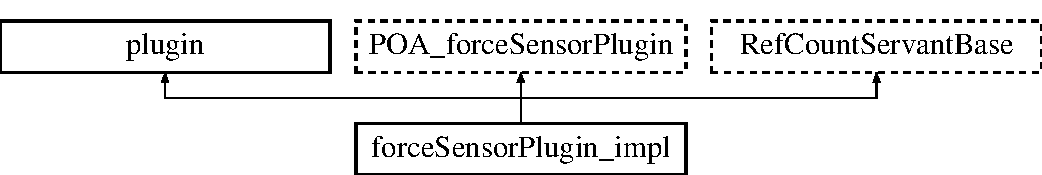
\includegraphics[height=2.000000cm]{classforceSensorPlugin__impl}
\end{center}
\end{figure}
\subsection*{Public Member Functions}
\begin{DoxyCompactItemize}
\item 
\hypertarget{classforceSensorPlugin__impl_ae7f2caafa5e19053c5d6c8b7d709a9d8}{void {\bfseries test} ()}\label{classforceSensorPlugin__impl_ae7f2caafa5e19053c5d6c8b7d709a9d8}

\item 
\hypertarget{classforceSensorPlugin__impl_a81bdec7eb5ce41b6342f0065754d451a}{{\bfseries force\-Sensor\-Plugin\-\_\-impl} (istringstream \&strm)}\label{classforceSensorPlugin__impl_a81bdec7eb5ce41b6342f0065754d451a}

\item 
\hypertarget{classforceSensorPlugin__impl_af36d740b9ac2d1aba8a2ed154c9dda48}{bool {\bfseries setup} (Robot\-State $\ast$rs, Robot\-State $\ast$mc)}\label{classforceSensorPlugin__impl_af36d740b9ac2d1aba8a2ed154c9dda48}

\item 
\hypertarget{classforceSensorPlugin__impl_abde11c5b0c37806e484d22640a334d8c}{void {\bfseries control} (Robot\-State $\ast$rs, Robot\-State $\ast$mc)}\label{classforceSensorPlugin__impl_abde11c5b0c37806e484d22640a334d8c}

\item 
\hypertarget{classforceSensorPlugin__impl_afb719dc4e48bd1fda7231b86e5497203}{bool {\bfseries cleanup} (Robot\-State $\ast$rs, Robot\-State $\ast$mc)}\label{classforceSensorPlugin__impl_afb719dc4e48bd1fda7231b86e5497203}

\end{DoxyCompactItemize}


The documentation for this class was generated from the following files\-:\begin{DoxyCompactItemize}
\item 
force\-Sensor\-Plugin\-\_\-impl.\-h\item 
force\-Sensor\-Plugin\-\_\-impl.\-cpp\end{DoxyCompactItemize}

\hypertarget{classhiroArm}{\section{hiro\-Arm Class Reference}
\label{classhiroArm}\index{hiro\-Arm@{hiro\-Arm}}
}
Inheritance diagram for hiro\-Arm\-:\begin{figure}[H]
\begin{center}
\leavevmode
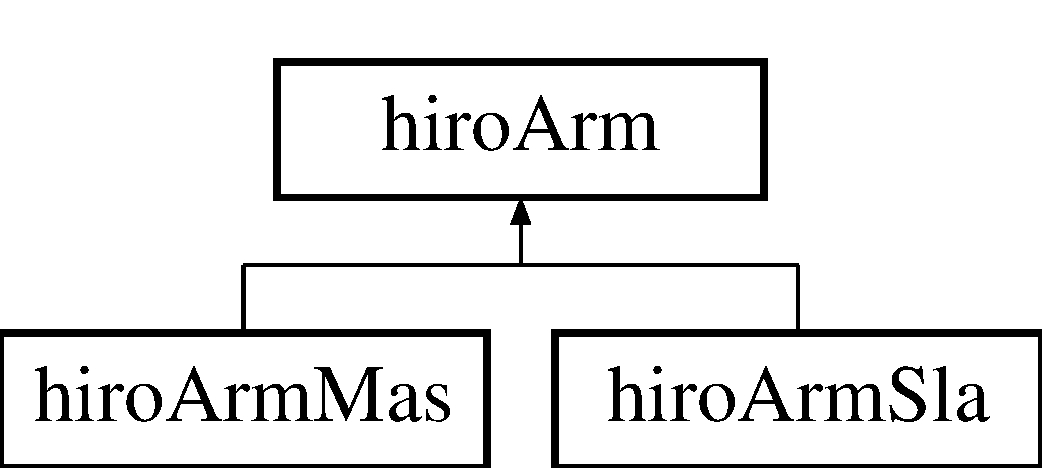
\includegraphics[height=2.000000cm]{classhiroArm}
\end{center}
\end{figure}
\subsection*{Classes}
\begin{DoxyCompactItemize}
\item 
struct \hyperlink{structhiroArm_1_1path__params}{path\-\_\-params}
\end{DoxyCompactItemize}
\subsection*{Public Types}
\begin{DoxyCompactItemize}
\item 
enum {\bfseries interpolation} \{ {\bfseries C\-O\-N\-S\-T\-A\-N\-T\-\_\-\-V\-E\-L\-O\-C\-I\-T\-Y}, 
{\bfseries Q\-U\-I\-N\-T\-I\-C\-\_\-\-F\-U\-N\-C\-T\-I\-O\-N}, 
{\bfseries E\-N\-D\-\_\-\-O\-F\-\_\-\-I\-N\-T\-E\-R\-P\-O\-L\-A\-T\-I\-O\-N}
 \}
\item 
enum {\bfseries cmode} \{ {\bfseries N\-O\-C\-O\-N\-T\-R\-O\-L}, 
{\bfseries V\-E\-L\-\_\-\-C\-O\-N\-T\-R\-O\-L}, 
{\bfseries I\-M\-P\-\_\-\-C\-O\-N\-T\-R\-O\-L}
 \}
\item 
enum \{ {\bfseries X}, 
{\bfseries Y}, 
{\bfseries Z}
 \}
\end{DoxyCompactItemize}
\subsection*{Public Member Functions}
\begin{DoxyCompactItemize}
\item 
\hypertarget{classhiroArm_a8e4aa1fa1e81ce07ee78c00b63c1bd54}{{\bfseries hiro\-Arm} (std\-::string name\-\_\-in, Body\-Ptr body\-\_\-in, unsigned int num\-\_\-q0\-\_\-in, double period\-\_\-in, float ang\-\_\-limits\-\_\-in\mbox{[}6\mbox{]}\mbox{[}5\mbox{]}, vector3 e\-Ph\-\_\-in, matrix33 e\-Rh\-\_\-in, vector3 h\-Pfs\-\_\-in)}\label{classhiroArm_a8e4aa1fa1e81ce07ee78c00b63c1bd54}

\item 
\hypertarget{classhiroArm_a2022d79b77c7e9d7c6c6b5418c450f66}{void {\bfseries init} ()}\label{classhiroArm_a2022d79b77c7e9d7c6c6b5418c450f66}

\item 
\hypertarget{classhiroArm_ab4818ca8441e606c3de5a1042c1a7452}{int {\bfseries init} (vector3 pos, matrix33 rot, double Cur\-Angles\mbox{[}15\mbox{]})}\label{classhiroArm_ab4818ca8441e606c3de5a1042c1a7452}

\item 
\hypertarget{classhiroArm_afa4bdab3188a17b39a9b943f22906eda}{virtual void {\bfseries savedata} ()}\label{classhiroArm_afa4bdab3188a17b39a9b943f22906eda}

\item 
\hypertarget{classhiroArm_a872988ae2b0ae8691c22c9eb8f7edb71}{std\-::string {\bfseries get\-\_\-name} ()}\label{classhiroArm_a872988ae2b0ae8691c22c9eb8f7edb71}

\item 
\hypertarget{classhiroArm_a9c17f63feaa2e08fd3ee0c8a7c1f8695}{void {\bfseries update\-\_\-currposdata} ()}\label{classhiroArm_a9c17f63feaa2e08fd3ee0c8a7c1f8695}

\item 
\hypertarget{classhiroArm_a2a6fff95ed7880b00f6fde6f587e1567}{void {\bfseries wrist2\-End\-Eff\-Xform} (vector3 r\-Pe, matrix33 r\-Re, vector3 \&r\-Ph, matrix33 \&r\-Rh)}\label{classhiroArm_a2a6fff95ed7880b00f6fde6f587e1567}

\item 
\hypertarget{classhiroArm_af30f07bdc11e6ead92e16ecc05fa01ae}{void {\bfseries End\-Eff2wrist\-Xform} (vector3 r\-Ph, matrix33 r\-Rh, vector3 \&r\-Pe)}\label{classhiroArm_af30f07bdc11e6ead92e16ecc05fa01ae}

\item 
\hypertarget{classhiroArm_a380c4809951756d76465a27925b81fb6}{dvector6 {\bfseries get\-\_\-qref} ()}\label{classhiroArm_a380c4809951756d76465a27925b81fb6}

\item 
\hypertarget{classhiroArm_a2b8e0d26de85f1b49bc178459f876f61}{dvector6 {\bfseries get\-\_\-qcur} ()}\label{classhiroArm_a2b8e0d26de85f1b49bc178459f876f61}

\item 
\hypertarget{classhiroArm_af33d770dbf20d3e9407db14381ca934b}{virtual void {\bfseries update\-\_\-currforcedata} ()}\label{classhiroArm_af33d770dbf20d3e9407db14381ca934b}

\item 
\hypertarget{classhiroArm_a82892b999ba5b188a77b7366fce27b0b}{virtual bool {\bfseries get\-\_\-forces} (vector3 \&r\-Fh\-\_\-gc\-\_\-out, vector3 \&r\-Mh\-\_\-gc\-\_\-out)}\label{classhiroArm_a82892b999ba5b188a77b7366fce27b0b}

\item 
\hypertarget{classhiroArm_afc2257c0efdfe06b05a5966e9953d919}{void {\bfseries get\-\_\-curr\-\_\-handpos} (vector3 \&r\-Ph\-\_\-out, matrix33 \&r\-Rh\-\_\-out)}\label{classhiroArm_afc2257c0efdfe06b05a5966e9953d919}

\item 
\hypertarget{classhiroArm_a925d818b5dca38fc993dd4935ffaade7}{void {\bfseries get\-\_\-ref\-\_\-handpos} (vector3 \&r\-Ph\-\_\-ref\-\_\-out, matrix33 \&r\-Rh\-\_\-ref\-\_\-out)}\label{classhiroArm_a925d818b5dca38fc993dd4935ffaade7}

\item 
\hypertarget{classhiroArm_a644d8a1a404c23fc512ebc6bf17a2f6c}{void {\bfseries set\-\_\-ref\-\_\-handpos} (vector3 r\-Ph\-\_\-ref\-\_\-in, matrix33 r\-Rh\-\_\-ref\-\_\-in)}\label{classhiroArm_a644d8a1a404c23fc512ebc6bf17a2f6c}

\item 
\hypertarget{classhiroArm_aeb0b11fd5c46fea119bf325b92daf5ca}{unsigned long {\bfseries get\-\_\-\-Iteration} ()}\label{classhiroArm_aeb0b11fd5c46fea119bf325b92daf5ca}

\item 
\hypertarget{classhiroArm_a7868ece4df8731426eaf7d46993c4145}{void {\bfseries set\-\_\-\-Iteration} ()}\label{classhiroArm_a7868ece4df8731426eaf7d46993c4145}

\item 
\hypertarget{classhiroArm_a4981564d8047b98beae3e25f0f67572e}{bool {\bfseries velocity\-\_\-control} (vector3 rd\-P, vector3 r\-W, bool f\-\_\-new)}\label{classhiroArm_a4981564d8047b98beae3e25f0f67572e}

\item 
\hypertarget{classhiroArm_ad68b57442891450fb9029e8c5d14520b}{bool {\bfseries impedance\-\_\-control} ()}\label{classhiroArm_ad68b57442891450fb9029e8c5d14520b}

\item 
\hypertarget{classhiroArm_aea4777c186d2f7de31439eeadcc2f34d}{void {\bfseries reset\-\_\-gravity\-\_\-comp} ()}\label{classhiroArm_aea4777c186d2f7de31439eeadcc2f34d}

\item 
\hypertarget{classhiroArm_a6a90d46b343f50a5e23a697606f3885d}{int {\bfseries gravity\-\_\-comp} ()}\label{classhiroArm_a6a90d46b343f50a5e23a697606f3885d}

\item 
\hypertarget{classhiroArm_af199c4ebb0f45666641f5ed5fb2cc833}{int {\bfseries moveto\-\_\-q\-\_\-goal} (dvector6 q\-\_\-goal\-\_\-in)}\label{classhiroArm_af199c4ebb0f45666641f5ed5fb2cc833}

\item 
\hypertarget{classhiroArm_af8abb5abd3a346325051b810d81ba4a8}{int {\bfseries Pivot\-Approach} (double cur\-\_\-time, vector3 pos, matrix33 rot, dvector6 curr\-Forces, dvector6 \&Joint\-Angle\-Update, dvector6 \&Curr\-Angles)}\label{classhiroArm_af8abb5abd3a346325051b810d81ba4a8}

\item 
\hypertarget{classhiroArm_a672283bbf662fc98c7034de8e01799d7}{void {\bfseries set\-\_\-\-Org\-Pos\-Rot} (vector3 \&pos, vector3 \&R\-P\-Y)}\label{classhiroArm_a672283bbf662fc98c7034de8e01799d7}

\end{DoxyCompactItemize}
\subsection*{Public Attributes}
\begin{DoxyCompactItemize}
\item 
\hypertarget{classhiroArm_a6a1070bcf7e873067785588c1fd31acc}{char {\bfseries Traj\-State1} \mbox{[}S\-T\-R\-\_\-\-L\-E\-N\mbox{]}}\label{classhiroArm_a6a1070bcf7e873067785588c1fd31acc}

\item 
\hypertarget{classhiroArm_a7dd8e40171e845af93566d2b054e07d8}{char {\bfseries Traj\-State2} \mbox{[}S\-T\-R\-\_\-\-L\-E\-N\mbox{]}}\label{classhiroArm_a7dd8e40171e845af93566d2b054e07d8}

\item 
\hypertarget{classhiroArm_a83700806446c3d2bc8e507aab3f49ff4}{char {\bfseries Angles} \mbox{[}S\-T\-R\-\_\-\-L\-E\-N\mbox{]}}\label{classhiroArm_a83700806446c3d2bc8e507aab3f49ff4}

\item 
\hypertarget{classhiroArm_a16f1798c82069ba29e316e69f5058134}{char {\bfseries Cart\-Pos} \mbox{[}S\-T\-R\-\_\-\-L\-E\-N\mbox{]}}\label{classhiroArm_a16f1798c82069ba29e316e69f5058134}

\item 
\hypertarget{classhiroArm_ad0877c20e534f3575cd18461e053fa4b}{char {\bfseries Forces} \mbox{[}S\-T\-R\-\_\-\-L\-E\-N\mbox{]}}\label{classhiroArm_ad0877c20e534f3575cd18461e053fa4b}

\item 
\hypertarget{classhiroArm_a9a1cb754cb1e4ab7f528a6d783a0fc81}{char {\bfseries State} \mbox{[}S\-T\-R\-\_\-\-L\-E\-N\mbox{]}}\label{classhiroArm_a9a1cb754cb1e4ab7f528a6d783a0fc81}

\item 
\hypertarget{classhiroArm_ab35146d2363f9be3b5a5268580b66cf2}{char {\bfseries manip\-Test} \mbox{[}S\-T\-R\-\_\-\-L\-E\-N\mbox{]}}\label{classhiroArm_ab35146d2363f9be3b5a5268580b66cf2}

\end{DoxyCompactItemize}
\subsection*{Protected Member Functions}
\begin{DoxyCompactItemize}
\item 
\hypertarget{classhiroArm_aba39f63dd2153875add31e519c4f0bec}{bool {\bfseries is\-\_\-moving} ()}\label{classhiroArm_aba39f63dd2153875add31e519c4f0bec}

\item 
\hypertarget{classhiroArm_acbab538d5731a0ca75ce8ea0a1655e2a}{bool {\bfseries is\-\_\-reached} ()}\label{classhiroArm_acbab538d5731a0ca75ce8ea0a1655e2a}

\item 
\hypertarget{classhiroArm_a1b8d50022eda626bd07d3a054955aef0}{bool {\bfseries is\-\_\-activated} ()}\label{classhiroArm_a1b8d50022eda626bd07d3a054955aef0}

\item 
\hypertarget{classhiroArm_ab36d0bde0961fbcecd52f4c7fff7451d}{bool {\bfseries init\-\_\-path\-\_\-params} (dvector6 q\-\_\-start\-\_\-in, dvector6 q\-\_\-goal\-\_\-in)}\label{classhiroArm_ab36d0bde0961fbcecd52f4c7fff7451d}

\item 
\hypertarget{classhiroArm_a49540d781f6413b08a1d8dfd712a92c4}{bool {\bfseries set\-\_\-path\-\_\-params} (\hyperlink{structhiroArm_1_1path__params}{path\-\_\-params} param\-\_\-in)}\label{classhiroArm_a49540d781f6413b08a1d8dfd712a92c4}

\item 
\hypertarget{classhiroArm_ab06838ff1aba7110ab0db0a7097e2a9a}{bool {\bfseries set\-\_\-path\-\_\-method} (interpolation method\-\_\-in)}\label{classhiroArm_ab06838ff1aba7110ab0db0a7097e2a9a}

\item 
\hypertarget{classhiroArm_a941f7eeda27141a3efdaee615fe59fb8}{bool {\bfseries set\-\_\-path\-\_\-max\-\_\-jvel} (double max\-\_\-jvel\-\_\-in)}\label{classhiroArm_a941f7eeda27141a3efdaee615fe59fb8}

\item 
\hypertarget{classhiroArm_a49ac0e06be2efc2028f29140795f7805}{bool {\bfseries calc\-\_\-duration\-\_\-jvel} (dvector6 distance\-\_\-in, double max\-\_\-jvel\-\_\-in)}\label{classhiroArm_a49ac0e06be2efc2028f29140795f7805}

\item 
\hypertarget{classhiroArm_aec2145c201642786832db74c7f2017b7}{bool {\bfseries calc\-\_\-qref} (vector3 r\-Ph\-\_\-ref\-\_\-in, matrix33 r\-Rh\-\_\-ref\-\_\-in, dvector6 \&q\-\_\-out)}\label{classhiroArm_aec2145c201642786832db74c7f2017b7}

\item 
\hypertarget{classhiroArm_a622b43c617ed85535a64554da180656a}{bool {\bfseries moveto} (dvector6 q\-\_\-start, dvector6 q\-\_\-goal)}\label{classhiroArm_a622b43c617ed85535a64554da180656a}

\item 
\hypertarget{classhiroArm_a1c2bbb832e890edf23688c71ed8c82e5}{bool {\bfseries calc\-\_\-gravity\-\_\-param} ()}\label{classhiroArm_a1c2bbb832e890edf23688c71ed8c82e5}

\item 
\hypertarget{classhiroArm_af221fa96d8de9e91509968d662187b30}{bool {\bfseries calc\-\_\-gravity\-\_\-param\-\_\-shimizu} ()}\label{classhiroArm_af221fa96d8de9e91509968d662187b30}

\item 
\hypertarget{classhiroArm_aa035fbbcf375297b8f6b9b8aab3b3449}{bool {\bfseries get\-\_\-raw\-\_\-forces} (double f\-\_\-out\mbox{[}6\mbox{]})}\label{classhiroArm_aa035fbbcf375297b8f6b9b8aab3b3449}

\item 
\hypertarget{classhiroArm_a2a162f14cb921ab87dec1fcf232c940f}{bool {\bfseries calc\-\_\-gc\-\_\-forces} (vector3 \&r\-Ffs\-\_\-gc\-\_\-out, vector3 \&r\-Mfs\-\_\-gc\-\_\-out)}\label{classhiroArm_a2a162f14cb921ab87dec1fcf232c940f}

\item 
\hypertarget{classhiroArm_a8ac00b1425ab54695392faa680041afb}{void {\bfseries calc\-\_\-gc\-\_\-forces\-\_\-at\-\_\-hand} (vector3 \&r\-Fh\-\_\-out, vector3 \&r\-Mh\-\_\-out)}\label{classhiroArm_a8ac00b1425ab54695392faa680041afb}

\item 
\hypertarget{classhiroArm_a6cd28378febc58968e53df0eed7deb35}{virtual matrix33 {\bfseries calc\-\_\-h\-Rfs} (dvector6 q\-\_\-in)}\label{classhiroArm_a6cd28378febc58968e53df0eed7deb35}

\item 
\hypertarget{classhiroArm_a5347280b572117eb0cd107e75df719e6}{void {\bfseries Skew\-To\-Vector} (matrix33 skew, vector3 \&vec)}\label{classhiroArm_a5347280b572117eb0cd107e75df719e6}

\item 
\hypertarget{classhiroArm_a67ebada1070014e309c3adc5953598f5}{matrix33 {\bfseries get\-\_\-rot33} (int dir, double rad)}\label{classhiroArm_a67ebada1070014e309c3adc5953598f5}

\item 
\hypertarget{classhiroArm_a234918c695614fa407e93597f6c6f4ee}{void {\bfseries calc\-\_\-r\-Pe\-\_\-r\-Re} (vector3 r\-Ph\-\_\-in, matrix33 r\-Rh\-\_\-in, vector3 \&r\-Pe\-\_\-out, matrix33 \&r\-Re\-\_\-out)}\label{classhiroArm_a234918c695614fa407e93597f6c6f4ee}

\end{DoxyCompactItemize}
\subsection*{Protected Attributes}
\begin{DoxyCompactItemize}
\item 
\hypertarget{classhiroArm_addf692c1741fb65d44a5147b072080ad}{\hyperlink{classAssemblyStrategy}{Assembly\-Strategy} $\ast$ {\bfseries P\-A}}\label{classhiroArm_addf692c1741fb65d44a5147b072080ad}

\item 
\hypertarget{classhiroArm_a7a1dcb206f544506a6a7682db98c8aff}{cmode {\bfseries controlmode}}\label{classhiroArm_a7a1dcb206f544506a6a7682db98c8aff}

\item 
\hypertarget{classhiroArm_a0bc88a2b6dc047e02f699ee83e13c970}{std\-::string {\bfseries name}}\label{classhiroArm_a0bc88a2b6dc047e02f699ee83e13c970}

\item 
\hypertarget{classhiroArm_a7686852c3087e04ffaacef6d9debd7df}{F\-I\-L\-E $\ast$ {\bfseries fp1}}\label{classhiroArm_a7686852c3087e04ffaacef6d9debd7df}

\item 
\hypertarget{classhiroArm_aa76ae3687822d66ac1c15767554378b1}{F\-I\-L\-E $\ast$ {\bfseries fp2}}\label{classhiroArm_aa76ae3687822d66ac1c15767554378b1}

\item 
\hypertarget{classhiroArm_a667d57ad53e218575ea5bf46c47835f1}{F\-I\-L\-E $\ast$ {\bfseries fp3}}\label{classhiroArm_a667d57ad53e218575ea5bf46c47835f1}

\item 
\hypertarget{classhiroArm_a9be626fdf0d7f8ad5ccfe1e58bf71cd8}{Body\-Ptr {\bfseries body}}\label{classhiroArm_a9be626fdf0d7f8ad5ccfe1e58bf71cd8}

\item 
\hypertarget{classhiroArm_a1c0a635880d06a60e71013a18ea73393}{Joint\-Path\-Ptr {\bfseries m\-\_\-path}}\label{classhiroArm_a1c0a635880d06a60e71013a18ea73393}

\item 
\hypertarget{classhiroArm_add995501c585c84318f106f8e75a93ef}{dvector6 {\bfseries q}}\label{classhiroArm_add995501c585c84318f106f8e75a93ef}

\item 
\hypertarget{classhiroArm_a52c93832cabb8ee2ff3fc04bc2281c39}{float {\bfseries ang\-\_\-limits} \mbox{[}A\-R\-M\-\_\-\-D\-O\-F\mbox{]}\mbox{[}5\mbox{]}}\label{classhiroArm_a52c93832cabb8ee2ff3fc04bc2281c39}

\item 
\hypertarget{classhiroArm_ad32280871291b28820114e9b72a0ac15}{unsigned int {\bfseries N\-U\-M\-\_\-q0}}\label{classhiroArm_ad32280871291b28820114e9b72a0ac15}

\item 
\hypertarget{classhiroArm_ac1a3c195009f1a607943def35d4e237e}{int {\bfseries N\-O\-\_\-fs}}\label{classhiroArm_ac1a3c195009f1a607943def35d4e237e}

\item 
\hypertarget{classhiroArm_af9f5f50294484a7cf3729df6fd027352}{double {\bfseries D\-E\-L\-\_\-\-T}}\label{classhiroArm_af9f5f50294484a7cf3729df6fd027352}

\item 
\hypertarget{classhiroArm_aee90413cc1a27e2382d421a08a574773}{double {\bfseries ik\-Gains} \mbox{[}4\mbox{]}}\label{classhiroArm_aee90413cc1a27e2382d421a08a574773}

\item 
\hypertarget{classhiroArm_acb7c4bbbf9df67951546e0d862020c2b}{double {\bfseries ik\-Rot} \mbox{[}4\mbox{]}}\label{classhiroArm_acb7c4bbbf9df67951546e0d862020c2b}

\item 
\hypertarget{classhiroArm_a06862814081b7d949d3a5a2d3efe69f2}{double {\bfseries ik\-Trans} \mbox{[}4\mbox{]}}\label{classhiroArm_a06862814081b7d949d3a5a2d3efe69f2}

\item 
\hypertarget{classhiroArm_acfb74760ea80e0afea9bf3615eef52cd}{vector3 {\bfseries fs\-F\-\_\-raw}}\label{classhiroArm_acfb74760ea80e0afea9bf3615eef52cd}

\item 
\hypertarget{classhiroArm_a3b2c289f887ee0cbd710af63be6a2dda}{vector3 {\bfseries fs\-M\-\_\-raw}}\label{classhiroArm_a3b2c289f887ee0cbd710af63be6a2dda}

\item 
\hypertarget{classhiroArm_ad76581c307801d517c8f08ea802cafdc}{vector3 {\bfseries r\-Ffs\-\_\-gc}}\label{classhiroArm_ad76581c307801d517c8f08ea802cafdc}

\item 
\hypertarget{classhiroArm_afd70fbf8efc37f3524103e9c739ffa9f}{vector3 {\bfseries r\-Mfs\-\_\-gc}}\label{classhiroArm_afd70fbf8efc37f3524103e9c739ffa9f}

\item 
\hypertarget{classhiroArm_ae717c02433d2a19e16117cc866ad5137}{vector3 {\bfseries r\-Fh\-\_\-gc}}\label{classhiroArm_ae717c02433d2a19e16117cc866ad5137}

\item 
\hypertarget{classhiroArm_a9b4e8c012c678ffd325071768ba512c3}{vector3 {\bfseries r\-Mh\-\_\-gc}}\label{classhiroArm_a9b4e8c012c678ffd325071768ba512c3}

\item 
\hypertarget{classhiroArm_a7205a4296f819801c1dc409852340915}{vector3 {\bfseries e\-Ph}}\label{classhiroArm_a7205a4296f819801c1dc409852340915}

\item 
\hypertarget{classhiroArm_ac93214e9d9e05d2a1fbee6044f2cf397}{matrix33 {\bfseries e\-Rh}}\label{classhiroArm_ac93214e9d9e05d2a1fbee6044f2cf397}

\item 
\hypertarget{classhiroArm_a5c419d02397e7e900c7f11e7b80725e0}{vector3 {\bfseries h\-Pfs}}\label{classhiroArm_a5c419d02397e7e900c7f11e7b80725e0}

\item 
\hypertarget{classhiroArm_aacec4ffa271326850a8cfd8838862af5}{vector3 {\bfseries r\-Ph}}\label{classhiroArm_aacec4ffa271326850a8cfd8838862af5}

\item 
\hypertarget{classhiroArm_aac5f7430a9d58bcad151c3823ccba13a}{matrix33 {\bfseries r\-Rh}}\label{classhiroArm_aac5f7430a9d58bcad151c3823ccba13a}

\item 
\hypertarget{classhiroArm_ae0c0b0806516ea795ecb482e58d7e0cc}{vector3 {\bfseries r\-Pe}}\label{classhiroArm_ae0c0b0806516ea795ecb482e58d7e0cc}

\item 
\hypertarget{classhiroArm_a53de271b4f521b6421ffbafca6cc20b2}{matrix33 {\bfseries r\-Re}}\label{classhiroArm_a53de271b4f521b6421ffbafca6cc20b2}

\item 
\hypertarget{classhiroArm_aee1e2a7ecc0ebcb21a2703464550f933}{vector3 {\bfseries r\-Ph\-\_\-ref}}\label{classhiroArm_aee1e2a7ecc0ebcb21a2703464550f933}

\item 
\hypertarget{classhiroArm_a800c540a6850d2065728625a6856c0b9}{matrix33 {\bfseries r\-Rh\-\_\-ref}}\label{classhiroArm_a800c540a6850d2065728625a6856c0b9}

\item 
\hypertarget{classhiroArm_abe8d6d75828d51e31923ceeb00d0b72b}{vector3 {\bfseries r\-Pe\-\_\-ref}}\label{classhiroArm_abe8d6d75828d51e31923ceeb00d0b72b}

\item 
\hypertarget{classhiroArm_abb69b5e9965ee0cb5d4705e271aa51af}{matrix33 {\bfseries r\-Re\-\_\-ref}}\label{classhiroArm_abb69b5e9965ee0cb5d4705e271aa51af}

\item 
\hypertarget{classhiroArm_a637f456fea3e4a306994cb6bf4b65759}{dvector6 {\bfseries q\-\_\-ref}}\label{classhiroArm_a637f456fea3e4a306994cb6bf4b65759}

\item 
\hypertarget{classhiroArm_a9a7363e208e5eadb3ed2c6c94adbce32}{bool {\bfseries f\-\_\-moving}}\label{classhiroArm_a9a7363e208e5eadb3ed2c6c94adbce32}

\item 
\hypertarget{classhiroArm_a8ea0beb035a51209bfe801e0614b6c74}{bool {\bfseries f\-\_\-reached}}\label{classhiroArm_a8ea0beb035a51209bfe801e0614b6c74}

\item 
\hypertarget{classhiroArm_a46befb8e4bc9374a40bc0fa97013b986}{unsigned long {\bfseries m\-\_\-time}}\label{classhiroArm_a46befb8e4bc9374a40bc0fa97013b986}

\item 
\hypertarget{classhiroArm_af2a99c1e0c9b1d8f6e601f89796848d7}{\hyperlink{structhiroArm_1_1path__params}{path\-\_\-params} {\bfseries p\-\_\-param}}\label{classhiroArm_af2a99c1e0c9b1d8f6e601f89796848d7}

\item 
\hypertarget{classhiroArm_adcc05d7df10344ed286712ac09e3bf36}{const double {\bfseries M\-A\-X\-\_\-\-J\-V\-E\-L}}\label{classhiroArm_adcc05d7df10344ed286712ac09e3bf36}

\item 
\hypertarget{classhiroArm_a13b1550abc6060781cf241ca51f6e1b8}{const double {\bfseries T\-I\-M\-E\-\_\-\-L\-I\-M\-I\-T}}\label{classhiroArm_a13b1550abc6060781cf241ca51f6e1b8}

\item 
\hypertarget{classhiroArm_a8fc0203fb50b15ee16cb30a907de9c91}{const double {\bfseries M\-I\-N\-\_\-\-P\-E\-R\-I\-O\-D}}\label{classhiroArm_a8fc0203fb50b15ee16cb30a907de9c91}

\item 
\hypertarget{classhiroArm_ac8b27c7b29aedb40a9703c838b39da47}{const double {\bfseries T\-O\-L\-E\-R\-A\-N\-C\-E}}\label{classhiroArm_ac8b27c7b29aedb40a9703c838b39da47}

\item 
\hypertarget{classhiroArm_aa2b4d94604d1a4d1c08141c16a64cd17}{matrix33 {\bfseries Mt}}\label{classhiroArm_aa2b4d94604d1a4d1c08141c16a64cd17}

\item 
\hypertarget{classhiroArm_a08986ace6f5dc9238bd00c92802cab19}{matrix33 {\bfseries Mr}}\label{classhiroArm_a08986ace6f5dc9238bd00c92802cab19}

\item 
\hypertarget{classhiroArm_a4fa6232e809edc31ee4597f019ed3923}{matrix33 {\bfseries Dt}}\label{classhiroArm_a4fa6232e809edc31ee4597f019ed3923}

\item 
\hypertarget{classhiroArm_ac5dd65ebd3ab4e25c965578517afe079}{matrix33 {\bfseries Dr}}\label{classhiroArm_ac5dd65ebd3ab4e25c965578517afe079}

\item 
\hypertarget{classhiroArm_a6dca906ca642c0a6e4cd753b63941586}{vector3 {\bfseries r\-Xd}}\label{classhiroArm_a6dca906ca642c0a6e4cd753b63941586}

\item 
\hypertarget{classhiroArm_af80787386161e59756a858c904f60e93}{vector3 {\bfseries rd\-Xd}}\label{classhiroArm_af80787386161e59756a858c904f60e93}

\item 
\hypertarget{classhiroArm_a90620d89f728c298c1e9ce7f4f863acc}{vector3 {\bfseries rdd\-Xd}}\label{classhiroArm_a90620d89f728c298c1e9ce7f4f863acc}

\item 
\hypertarget{classhiroArm_a51e3d336896d807590df5b48d29c5532}{vector3 {\bfseries r\-Rd}}\label{classhiroArm_a51e3d336896d807590df5b48d29c5532}

\item 
\hypertarget{classhiroArm_a4235bbdf7465a884581d91e51862787d}{vector3 {\bfseries rd\-Rd}}\label{classhiroArm_a4235bbdf7465a884581d91e51862787d}

\item 
\hypertarget{classhiroArm_a64bd2ff702c6e38b4ea2986e6b796e28}{vector3 {\bfseries rdd\-Rd}}\label{classhiroArm_a64bd2ff702c6e38b4ea2986e6b796e28}

\item 
\hypertarget{classhiroArm_ab33ad5f1ceb707325583fe9e10261cc3}{bool {\bfseries f\-\_\-gc}}\label{classhiroArm_ab33ad5f1ceb707325583fe9e10261cc3}

\item 
\hypertarget{classhiroArm_a16ec70d24b26dcbbfda883ad96afa7b6}{bool {\bfseries f\-\_\-gc\-\_\-init}}\label{classhiroArm_a16ec70d24b26dcbbfda883ad96afa7b6}

\item 
\hypertarget{classhiroArm_a485b8d223930c7dd9fb3139cc89f24df}{int {\bfseries step\-\_\-gc}}\label{classhiroArm_a485b8d223930c7dd9fb3139cc89f24df}

\item 
\hypertarget{classhiroArm_a51548d7ac2193834a23abaf48bfe05fc}{int {\bfseries step\-\_\-fs}}\label{classhiroArm_a51548d7ac2193834a23abaf48bfe05fc}

\item 
\hypertarget{classhiroArm_a6a280e8faf8d065344373c264db0d65d}{double {\bfseries mass}}\label{classhiroArm_a6a280e8faf8d065344373c264db0d65d}

\item 
\hypertarget{classhiroArm_ab198cbb1cdaf345f27a225d314240e06}{const int {\bfseries max\-\_\-step\-\_\-fs}}\label{classhiroArm_ab198cbb1cdaf345f27a225d314240e06}

\item 
\hypertarget{classhiroArm_a77b52da322594e9d6ffbfd5203fa43bc}{const int {\bfseries wait\-\_\-step}}\label{classhiroArm_a77b52da322594e9d6ffbfd5203fa43bc}

\item 
\hypertarget{classhiroArm_a9d73a120be971c2bf9d75e7b2650c819}{const double {\bfseries G\-A\-C\-C}}\label{classhiroArm_a9d73a120be971c2bf9d75e7b2650c819}

\item 
\hypertarget{classhiroArm_a2832693d428ea1eb2ec38fc87094d063}{vector3 {\bfseries r\-G\-\_\-vec}}\label{classhiroArm_a2832693d428ea1eb2ec38fc87094d063}

\item 
\hypertarget{classhiroArm_ad013a710860c7e1808cd361b0e2cd0ab}{vector3 {\bfseries fs\-Pgc}}\label{classhiroArm_ad013a710860c7e1808cd361b0e2cd0ab}

\item 
\hypertarget{classhiroArm_aacb04f805240685c6f28728ac407010c}{vector3 {\bfseries fs\-F\-\_\-offset}}\label{classhiroArm_aacb04f805240685c6f28728ac407010c}

\item 
\hypertarget{classhiroArm_afdff32f72a25a22319d634e37ca66cca}{vector3 {\bfseries fs\-M\-\_\-offset}}\label{classhiroArm_afdff32f72a25a22319d634e37ca66cca}

\item 
\hypertarget{classhiroArm_aa92bec0148891075371a6dce46377f4d}{vector3 {\bfseries fs\-F\-\_\-tmp} \mbox{[}5\mbox{]}}\label{classhiroArm_aa92bec0148891075371a6dce46377f4d}

\item 
\hypertarget{classhiroArm_a71e59362250b53e7fdd6a8eb43e13fdf}{vector3 {\bfseries fs\-M\-\_\-tmp} \mbox{[}5\mbox{]}}\label{classhiroArm_a71e59362250b53e7fdd6a8eb43e13fdf}

\item 
\hypertarget{classhiroArm_ac84c9861e6761231639f5a9f5178cb93}{dvector6 {\bfseries q\-\_\-gc\-\_\-ref} \mbox{[}5\mbox{]}}\label{classhiroArm_ac84c9861e6761231639f5a9f5178cb93}

\item 
\hypertarget{classhiroArm_a0e69681e3882555cc18ae8bd6191e535}{matrix33 {\bfseries fs\-Rr\-\_\-gc} \mbox{[}5\mbox{]}}\label{classhiroArm_a0e69681e3882555cc18ae8bd6191e535}

\item 
\hypertarget{classhiroArm_aaf7d09fbdea5bfe0ba41eb31761b6aed}{vector3 {\bfseries r\-Ph\-\_\-initial}}\label{classhiroArm_aaf7d09fbdea5bfe0ba41eb31761b6aed}

\item 
\hypertarget{classhiroArm_ad8ebd1440896701a3a44dbd16b06e79d}{matrix33 {\bfseries r\-Rh\-\_\-initial}}\label{classhiroArm_ad8ebd1440896701a3a44dbd16b06e79d}

\item 
\hypertarget{classhiroArm_a1503923eddd3cc2bbb996b5d9ed306e5}{vector3 {\bfseries fs\-F\-\_\-initial}}\label{classhiroArm_a1503923eddd3cc2bbb996b5d9ed306e5}

\item 
\hypertarget{classhiroArm_a27db0eb1157726a75cc0c760dbb984c9}{vector3 {\bfseries fs\-M\-\_\-initial}}\label{classhiroArm_a27db0eb1157726a75cc0c760dbb984c9}

\item 
\hypertarget{classhiroArm_af1aded47966174202506f75d464dab51}{std\-::ifstream {\bfseries fin\-\_\-lpos}}\label{classhiroArm_af1aded47966174202506f75d464dab51}

\item 
\hypertarget{classhiroArm_a336342501e46c62ee5f2021c3f44835c}{std\-::ifstream {\bfseries fin\-\_\-rpos}}\label{classhiroArm_a336342501e46c62ee5f2021c3f44835c}

\item 
\hypertarget{classhiroArm_a4106db25c02c7ca50d66ea943ff7e9ab}{std\-::ifstream {\bfseries fin\-\_\-lfc}}\label{classhiroArm_a4106db25c02c7ca50d66ea943ff7e9ab}

\item 
\hypertarget{classhiroArm_a4cf03d39eb6faa765bcc58090ea5a604}{std\-::ifstream {\bfseries fin\-\_\-rfc}}\label{classhiroArm_a4cf03d39eb6faa765bcc58090ea5a604}

\item 
\hypertarget{classhiroArm_a38fffc28b35466feb50467dd49282f1a}{bool {\bfseries init\-Flag}}\label{classhiroArm_a38fffc28b35466feb50467dd49282f1a}

\end{DoxyCompactItemize}
\subsection*{Friends}
\begin{DoxyCompactItemize}
\item 
\hypertarget{classhiroArm_a05deaa370806bc767b12f2aef37c348a}{class {\bfseries force\-Sensor\-Plugin\-\_\-impl}}\label{classhiroArm_a05deaa370806bc767b12f2aef37c348a}

\end{DoxyCompactItemize}


The documentation for this class was generated from the following files\-:\begin{DoxyCompactItemize}
\item 
\hyperlink{hiroArm_8h}{hiro\-Arm.\-h}\item 
\hyperlink{hiroArm_8cpp}{hiro\-Arm.\-cpp}\end{DoxyCompactItemize}

\hypertarget{classhiroArmMas}{\section{hiro\-Arm\-Mas Class Reference}
\label{classhiroArmMas}\index{hiro\-Arm\-Mas@{hiro\-Arm\-Mas}}
}
Inheritance diagram for hiro\-Arm\-Mas\-:\begin{figure}[H]
\begin{center}
\leavevmode
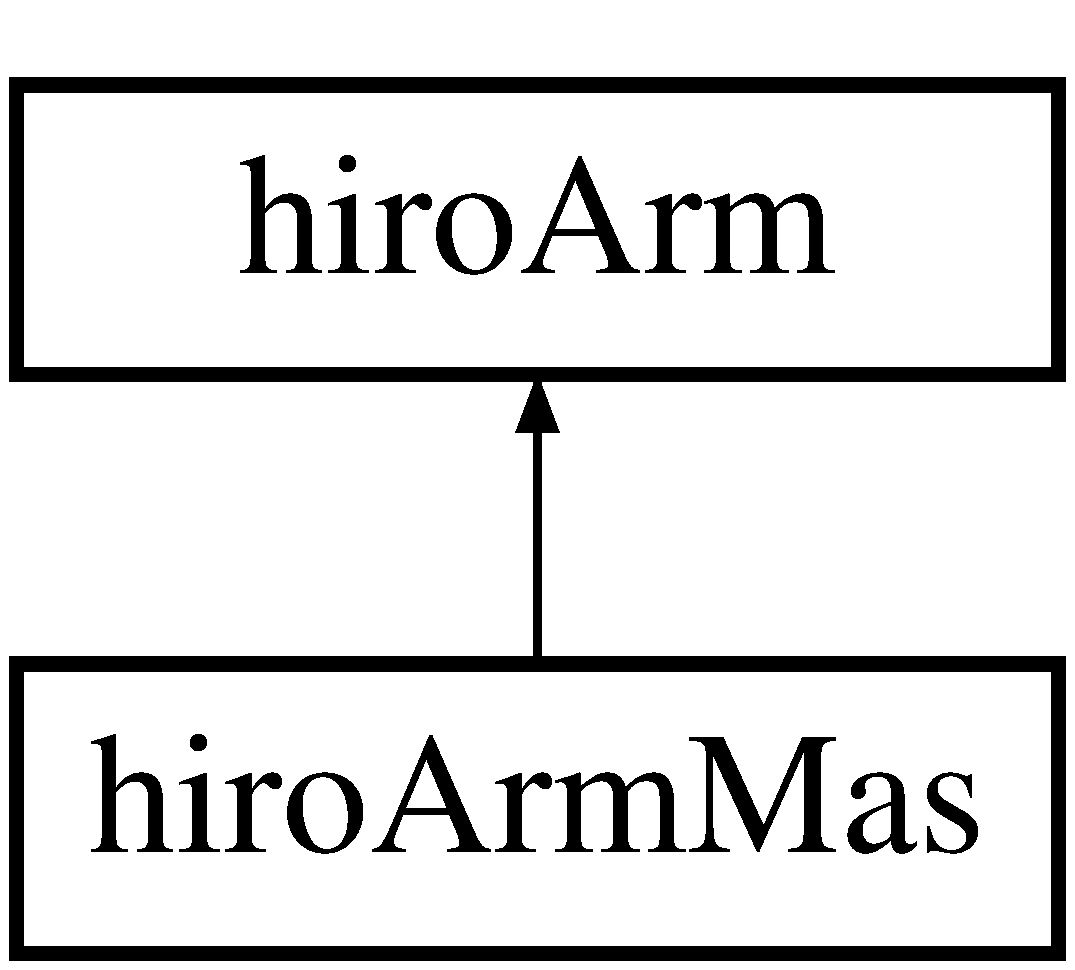
\includegraphics[height=2.000000cm]{classhiroArmMas}
\end{center}
\end{figure}
\subsection*{Public Member Functions}
\begin{DoxyCompactItemize}
\item 
\hypertarget{classhiroArmMas_aa665804de61cf4a7adf11ebe722611be}{{\bfseries hiro\-Arm\-Mas} (std\-::string name\-\_\-in, Body\-Ptr body\-\_\-in, unsigned int num\-\_\-q0\-\_\-in, double period\-\_\-in, float ang\-\_\-limits\-\_\-in\mbox{[}6\mbox{]}\mbox{[}5\mbox{]}, vector3 e\-Ph\-\_\-in, matrix33 e\-Rh\-\_\-in, vector3 h\-Pfs\-\_\-in)}\label{classhiroArmMas_aa665804de61cf4a7adf11ebe722611be}

\end{DoxyCompactItemize}
\subsection*{Protected Member Functions}
\begin{DoxyCompactItemize}
\item 
\hypertarget{classhiroArmMas_af1e337aade07c23bd776b9e923bacc46}{matrix33 {\bfseries calc\-\_\-h\-Rfs} (dvector6 q\-\_\-in)}\label{classhiroArmMas_af1e337aade07c23bd776b9e923bacc46}

\end{DoxyCompactItemize}
\subsection*{Additional Inherited Members}


The documentation for this class was generated from the following files\-:\begin{DoxyCompactItemize}
\item 
\hyperlink{hiroArm_8h}{hiro\-Arm.\-h}\item 
\hyperlink{hiroArm_8cpp}{hiro\-Arm.\-cpp}\end{DoxyCompactItemize}

\hypertarget{classhiroArmSla}{\section{hiro\-Arm\-Sla Class Reference}
\label{classhiroArmSla}\index{hiro\-Arm\-Sla@{hiro\-Arm\-Sla}}
}
Inheritance diagram for hiro\-Arm\-Sla\-:\begin{figure}[H]
\begin{center}
\leavevmode
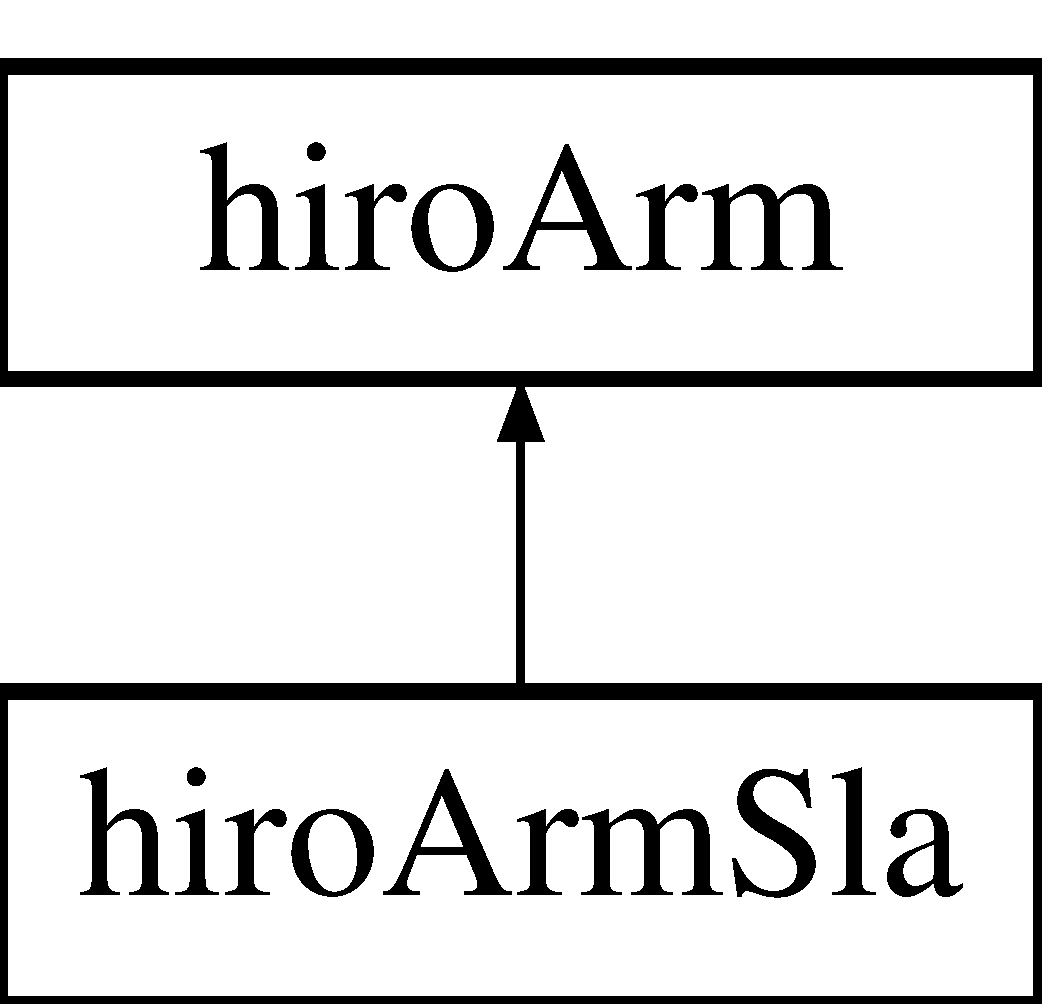
\includegraphics[height=2.000000cm]{classhiroArmSla}
\end{center}
\end{figure}
\subsection*{Public Member Functions}
\begin{DoxyCompactItemize}
\item 
\hypertarget{classhiroArmSla_a888535be8209d2d22dcc06147e29f6c2}{{\bfseries hiro\-Arm\-Sla} (std\-::string name\-\_\-in, Body\-Ptr body\-\_\-in, unsigned int num\-\_\-q0\-\_\-in, double period\-\_\-in, float ang\-\_\-limits\-\_\-in\mbox{[}6\mbox{]}\mbox{[}5\mbox{]}, vector3 e\-Ph\-\_\-in, matrix33 e\-Rh\-\_\-in, vector3 h\-Pfs\-\_\-in, matrix33 h\-Rfs\-\_\-in)}\label{classhiroArmSla_a888535be8209d2d22dcc06147e29f6c2}

\end{DoxyCompactItemize}
\subsection*{Protected Member Functions}
\begin{DoxyCompactItemize}
\item 
\hypertarget{classhiroArmSla_a5ea00712a02f096e568af6eadcdd51e9}{matrix33 {\bfseries calc\-\_\-h\-Rfs} (dvector6 q\-\_\-in)}\label{classhiroArmSla_a5ea00712a02f096e568af6eadcdd51e9}

\end{DoxyCompactItemize}
\subsection*{Protected Attributes}
\begin{DoxyCompactItemize}
\item 
\hypertarget{classhiroArmSla_aab7a8ab7ff319848bb35193668f76d6e}{matrix33 {\bfseries h\-Rfs}}\label{classhiroArmSla_aab7a8ab7ff319848bb35193668f76d6e}

\end{DoxyCompactItemize}
\subsection*{Additional Inherited Members}


The documentation for this class was generated from the following files\-:\begin{DoxyCompactItemize}
\item 
\hyperlink{hiroArm_8h}{hiro\-Arm.\-h}\item 
\hyperlink{hiroArm_8cpp}{hiro\-Arm.\-cpp}\end{DoxyCompactItemize}

\hypertarget{structOpenHRP_1_1CFSImpl_1_1LinkData}{\section{Open\-H\-R\-P\-:\-:C\-F\-S\-Impl\-:\-:Link\-Data Struct Reference}
\label{structOpenHRP_1_1CFSImpl_1_1LinkData}\index{Open\-H\-R\-P\-::\-C\-F\-S\-Impl\-::\-Link\-Data@{Open\-H\-R\-P\-::\-C\-F\-S\-Impl\-::\-Link\-Data}}
}
\subsection*{Public Attributes}
\begin{DoxyCompactItemize}
\item 
\hypertarget{structOpenHRP_1_1CFSImpl_1_1LinkData_aa4cf5b0652d098ab4ea2be1ecf1e3248}{vector3 {\bfseries dvo}}\label{structOpenHRP_1_1CFSImpl_1_1LinkData_aa4cf5b0652d098ab4ea2be1ecf1e3248}

\item 
\hypertarget{structOpenHRP_1_1CFSImpl_1_1LinkData_a69b0d0a51edc38cb72792b61404df10b}{vector3 {\bfseries dw}}\label{structOpenHRP_1_1CFSImpl_1_1LinkData_a69b0d0a51edc38cb72792b61404df10b}

\item 
\hypertarget{structOpenHRP_1_1CFSImpl_1_1LinkData_a48cae13aceaa53e7a05a175028c8054d}{vector3 {\bfseries pf0}}\label{structOpenHRP_1_1CFSImpl_1_1LinkData_a48cae13aceaa53e7a05a175028c8054d}

\item 
\hypertarget{structOpenHRP_1_1CFSImpl_1_1LinkData_a7e2ff763392947e7e96c68ab137cfcf3}{vector3 {\bfseries ptau0}}\label{structOpenHRP_1_1CFSImpl_1_1LinkData_a7e2ff763392947e7e96c68ab137cfcf3}

\item 
\hypertarget{structOpenHRP_1_1CFSImpl_1_1LinkData_a3ee72839018e17c7aea5963c39c0b314}{double {\bfseries uu}}\label{structOpenHRP_1_1CFSImpl_1_1LinkData_a3ee72839018e17c7aea5963c39c0b314}

\item 
\hypertarget{structOpenHRP_1_1CFSImpl_1_1LinkData_afc5a9926fc54b6866a2554553d89a0c2}{double {\bfseries uu0}}\label{structOpenHRP_1_1CFSImpl_1_1LinkData_afc5a9926fc54b6866a2554553d89a0c2}

\item 
\hypertarget{structOpenHRP_1_1CFSImpl_1_1LinkData_a786f7c7990d5e5f85ac3602d754c058f}{double {\bfseries ddq}}\label{structOpenHRP_1_1CFSImpl_1_1LinkData_a786f7c7990d5e5f85ac3602d754c058f}

\item 
\hypertarget{structOpenHRP_1_1CFSImpl_1_1LinkData_a82a0a28f6f7363416101f2f6f41e55a5}{int {\bfseries number\-To\-Check\-Accel\-Calc\-Skip}}\label{structOpenHRP_1_1CFSImpl_1_1LinkData_a82a0a28f6f7363416101f2f6f41e55a5}

\item 
\hypertarget{structOpenHRP_1_1CFSImpl_1_1LinkData_a5987d86a8029fd49bf630e7cb822f920}{int {\bfseries parent\-Index}}\label{structOpenHRP_1_1CFSImpl_1_1LinkData_a5987d86a8029fd49bf630e7cb822f920}

\item 
\hypertarget{structOpenHRP_1_1CFSImpl_1_1LinkData_a7bf17d5c4da24fc690fb8a6de3efa54d}{Link $\ast$ {\bfseries link}}\label{structOpenHRP_1_1CFSImpl_1_1LinkData_a7bf17d5c4da24fc690fb8a6de3efa54d}

\end{DoxyCompactItemize}


The documentation for this struct was generated from the following file\-:\begin{DoxyCompactItemize}
\item 
\hyperlink{ConstraintForceSolver_8cpp}{Constraint\-Force\-Solver.\-cpp}\end{DoxyCompactItemize}

\hypertarget{structOpenHRP_1_1CFSImpl_1_1LinkPair}{\section{Open\-H\-R\-P\-:\-:C\-F\-S\-Impl\-:\-:Link\-Pair Struct Reference}
\label{structOpenHRP_1_1CFSImpl_1_1LinkPair}\index{Open\-H\-R\-P\-::\-C\-F\-S\-Impl\-::\-Link\-Pair@{Open\-H\-R\-P\-::\-C\-F\-S\-Impl\-::\-Link\-Pair}}
}
\subsection*{Public Attributes}
\begin{DoxyCompactItemize}
\item 
\hypertarget{structOpenHRP_1_1CFSImpl_1_1LinkPair_a09c42e4d7acaca4f5221c33858a5eaf6}{int {\bfseries index}}\label{structOpenHRP_1_1CFSImpl_1_1LinkPair_a09c42e4d7acaca4f5221c33858a5eaf6}

\item 
\hypertarget{structOpenHRP_1_1CFSImpl_1_1LinkPair_a8653c3c7af8dcc93d497d71b8e4ef0d4}{bool {\bfseries is\-Same\-Body\-Pair}}\label{structOpenHRP_1_1CFSImpl_1_1LinkPair_a8653c3c7af8dcc93d497d71b8e4ef0d4}

\item 
\hypertarget{structOpenHRP_1_1CFSImpl_1_1LinkPair_a6e55e738107fa2c09fdfe7debdcb9a06}{int {\bfseries body\-Index} \mbox{[}2\mbox{]}}\label{structOpenHRP_1_1CFSImpl_1_1LinkPair_a6e55e738107fa2c09fdfe7debdcb9a06}

\item 
\hypertarget{structOpenHRP_1_1CFSImpl_1_1LinkPair_a2dbf8cc0babcdcc94f5eaac796afe9d1}{\hyperlink{structOpenHRP_1_1CFSImpl_1_1BodyData}{Body\-Data} $\ast$ {\bfseries body\-Data} \mbox{[}2\mbox{]}}\label{structOpenHRP_1_1CFSImpl_1_1LinkPair_a2dbf8cc0babcdcc94f5eaac796afe9d1}

\item 
\hypertarget{structOpenHRP_1_1CFSImpl_1_1LinkPair_ab2735b6201cb0d7aace0e646eabe36d2}{Link $\ast$ {\bfseries link} \mbox{[}2\mbox{]}}\label{structOpenHRP_1_1CFSImpl_1_1LinkPair_ab2735b6201cb0d7aace0e646eabe36d2}

\item 
\hypertarget{structOpenHRP_1_1CFSImpl_1_1LinkPair_aa30c2d83bec055bdfb182222857a7d3f}{\hyperlink{structOpenHRP_1_1CFSImpl_1_1LinkData}{Link\-Data} $\ast$ {\bfseries link\-Data} \mbox{[}2\mbox{]}}\label{structOpenHRP_1_1CFSImpl_1_1LinkPair_aa30c2d83bec055bdfb182222857a7d3f}

\item 
\hypertarget{structOpenHRP_1_1CFSImpl_1_1LinkPair_a78ae8f94fa5c18612d2f2cef2d8ea43f}{Constraint\-Point\-Array {\bfseries constraint\-Points}}\label{structOpenHRP_1_1CFSImpl_1_1LinkPair_a78ae8f94fa5c18612d2f2cef2d8ea43f}

\item 
\hypertarget{structOpenHRP_1_1CFSImpl_1_1LinkPair_a60f150ec293f131398a0b52deb3fea9f}{double {\bfseries mu\-Static}}\label{structOpenHRP_1_1CFSImpl_1_1LinkPair_a60f150ec293f131398a0b52deb3fea9f}

\item 
\hypertarget{structOpenHRP_1_1CFSImpl_1_1LinkPair_ad3972cddecc181e32ff54fd09d578666}{double {\bfseries mu\-Dynamic}}\label{structOpenHRP_1_1CFSImpl_1_1LinkPair_ad3972cddecc181e32ff54fd09d578666}

\item 
\hypertarget{structOpenHRP_1_1CFSImpl_1_1LinkPair_a2615eb6ee9e7492c168ae2062c6dd491}{double {\bfseries epsilon}}\label{structOpenHRP_1_1CFSImpl_1_1LinkPair_a2615eb6ee9e7492c168ae2062c6dd491}

\item 
\hypertarget{structOpenHRP_1_1CFSImpl_1_1LinkPair_a9f492145d36dacfb16dc202420c44ed7}{Body\-::\-Link\-Connection $\ast$ {\bfseries connection}}\label{structOpenHRP_1_1CFSImpl_1_1LinkPair_a9f492145d36dacfb16dc202420c44ed7}

\end{DoxyCompactItemize}


The documentation for this struct was generated from the following file\-:\begin{DoxyCompactItemize}
\item 
\hyperlink{ConstraintForceSolver_8cpp}{Constraint\-Force\-Solver.\-cpp}\end{DoxyCompactItemize}

\hypertarget{classnittaFS}{\section{nitta\-F\-S Class Reference}
\label{classnittaFS}\index{nitta\-F\-S@{nitta\-F\-S}}
}


{\ttfamily \#include $<$nitta\-F\-S.\-h$>$}

\subsection*{Public Member Functions}
\begin{DoxyCompactItemize}
\item 
\hypertarget{classnittaFS_abe00fd4b734087de242182663b403894}{bool {\bfseries init} ()}\label{classnittaFS_abe00fd4b734087de242182663b403894}

\item 
\hypertarget{classnittaFS_a3bc8d3fc4ff796dae47b276efceca5e2}{int {\bfseries get\-\_\-units} (int No, double units\mbox{[}3\mbox{]})}\label{classnittaFS_a3bc8d3fc4ff796dae47b276efceca5e2}

\item 
\hypertarget{classnittaFS_a4efc973bd9431d7b31b1975228ad3d37}{void {\bfseries set\-\_\-offset} (int No, int offsets\mbox{[}6\mbox{]})}\label{classnittaFS_a4efc973bd9431d7b31b1975228ad3d37}

\item 
\hypertarget{classnittaFS_a52bb8b23bcdbc38934d24fdc3f4a2a1e}{void {\bfseries get\-\_\-offset} (int No, int offsets\mbox{[}6\mbox{]})}\label{classnittaFS_a52bb8b23bcdbc38934d24fdc3f4a2a1e}

\item 
\hypertarget{classnittaFS_a0d416bb7c24fb2173cf7992812e2a34b}{void {\bfseries reset\-\_\-offset} (int No)}\label{classnittaFS_a0d416bb7c24fb2173cf7992812e2a34b}

\item 
\hypertarget{classnittaFS_a401d5e4716bbc8517a25427328776e52}{void {\bfseries get\-\_\-forces} (int No, double forces\mbox{[}6\mbox{]})}\label{classnittaFS_a401d5e4716bbc8517a25427328776e52}

\end{DoxyCompactItemize}
\subsection*{Protected Member Functions}
\begin{DoxyCompactItemize}
\item 
\hypertarget{classnittaFS_a3a63e33a5deac3dc632a16e1f05037c9}{short {\bfseries I\-F\-S\-\_\-\-Read} (unsigned long Mapped\-Address, unsigned int addr)}\label{classnittaFS_a3a63e33a5deac3dc632a16e1f05037c9}

\item 
\hypertarget{classnittaFS_ab64069e55cdfacfe27ec0c0a12bf5ff4}{void {\bfseries I\-F\-S\-\_\-\-Write} (unsigned long Mapped\-Address, unsigned int addr, int data)}\label{classnittaFS_ab64069e55cdfacfe27ec0c0a12bf5ff4}

\item 
\hypertarget{classnittaFS_abda0312459b432cd9481f3cd5819e51f}{int {\bfseries download} (unsigned int base0, unsigned int base1)}\label{classnittaFS_abda0312459b432cd9481f3cd5819e51f}

\end{DoxyCompactItemize}
\subsection*{Protected Attributes}
\begin{DoxyCompactItemize}
\item 
\hypertarget{classnittaFS_a152198679f024b41db4471a6e2f572d9}{unsigned long {\bfseries Mapped\-Address0}}\label{classnittaFS_a152198679f024b41db4471a6e2f572d9}

\item 
\hypertarget{classnittaFS_a47dc1731b82ee6a1030079f2179aaca4}{unsigned long {\bfseries Mapped\-Address1}}\label{classnittaFS_a47dc1731b82ee6a1030079f2179aaca4}

\item 
\hypertarget{classnittaFS_ada2d920bb8cc5b1f65adf5a4849b7e87}{int {\bfseries m\-\_\-offsets} \mbox{[}2\mbox{]}\mbox{[}6\mbox{]}}\label{classnittaFS_ada2d920bb8cc5b1f65adf5a4849b7e87}

\item 
\hypertarget{classnittaFS_a73ec958173112fd21a0f05d949117c4d}{int {\bfseries m\-\_\-unit\-\_\-no} \mbox{[}2\mbox{]}}\label{classnittaFS_a73ec958173112fd21a0f05d949117c4d}

\item 
\hypertarget{classnittaFS_a6504b0630bfaf141bafcb251a85cd4ed}{double {\bfseries m\-\_\-units} \mbox{[}2\mbox{]}\mbox{[}6\mbox{]}}\label{classnittaFS_a6504b0630bfaf141bafcb251a85cd4ed}

\end{DoxyCompactItemize}


\subsection{Detailed Description}
Res\-Mgr and Message Server Process

This program is for J\-R3/\-Nitta Force moment sensor. Copyright(\-C) by Waseda University, Nitta Coropration. 2002. modified by n-\/yamanobe 2011/02/16 

The documentation for this class was generated from the following files\-:\begin{DoxyCompactItemize}
\item 
\hyperlink{nittaFS_8h}{nitta\-F\-S.\-h}\item 
\hyperlink{nittaFS_8cpp}{nitta\-F\-S.\-cpp}\end{DoxyCompactItemize}

\hypertarget{structhiroArm_1_1path__params}{\section{hiro\-Arm\-:\-:path\-\_\-params Struct Reference}
\label{structhiroArm_1_1path__params}\index{hiro\-Arm\-::path\-\_\-params@{hiro\-Arm\-::path\-\_\-params}}
}
\subsection*{Public Attributes}
\begin{DoxyCompactItemize}
\item 
\hypertarget{structhiroArm_1_1path__params_a32faccf34e7ff3fdf7a1fd04b09473a3}{interpolation {\bfseries method}}\label{structhiroArm_1_1path__params_a32faccf34e7ff3fdf7a1fd04b09473a3}

\item 
\hypertarget{structhiroArm_1_1path__params_a5f0c5282fd7030b93d5e12c213868707}{double {\bfseries max\-\_\-jvel}}\label{structhiroArm_1_1path__params_a5f0c5282fd7030b93d5e12c213868707}

\item 
\hypertarget{structhiroArm_1_1path__params_aa4301fa0c840ebc0e486440309c0bd60}{dvector6 {\bfseries q\-\_\-start}}\label{structhiroArm_1_1path__params_aa4301fa0c840ebc0e486440309c0bd60}

\item 
\hypertarget{structhiroArm_1_1path__params_a1a5e3887d9e304fa72025371484dd21f}{dvector6 {\bfseries q\-\_\-goal}}\label{structhiroArm_1_1path__params_a1a5e3887d9e304fa72025371484dd21f}

\item 
\hypertarget{structhiroArm_1_1path__params_a0871678d0dd60e39dad49a3d130e56b8}{dvector6 {\bfseries distance}}\label{structhiroArm_1_1path__params_a0871678d0dd60e39dad49a3d130e56b8}

\item 
\hypertarget{structhiroArm_1_1path__params_af4ca58fa99d882f8d0fa5804360a0fce}{double {\bfseries duration}}\label{structhiroArm_1_1path__params_af4ca58fa99d882f8d0fa5804360a0fce}

\item 
\hypertarget{structhiroArm_1_1path__params_aedf0b1cb5a9cf6ee2bf21b961c44f354}{dvector6 {\bfseries jvel}}\label{structhiroArm_1_1path__params_aedf0b1cb5a9cf6ee2bf21b961c44f354}

\end{DoxyCompactItemize}


The documentation for this struct was generated from the following file\-:\begin{DoxyCompactItemize}
\item 
\hyperlink{hiroArm_8h}{hiro\-Arm.\-h}\end{DoxyCompactItemize}

\chapter{File Documentation}
\hypertarget{ConstraintForceSolver_8cpp}{\section{Constraint\-Force\-Solver.\-cpp File Reference}
\label{ConstraintForceSolver_8cpp}\index{Constraint\-Force\-Solver.\-cpp@{Constraint\-Force\-Solver.\-cpp}}
}


Implementation of Contact\-Force\-Solver class.  


{\ttfamily \#include \char`\"{}tvmet3d.\-h\char`\"{}}\\*
{\ttfamily \#include \char`\"{}World.\-h\char`\"{}}\\*
{\ttfamily \#include \char`\"{}Body.\-h\char`\"{}}\\*
{\ttfamily \#include \char`\"{}Link.\-h\char`\"{}}\\*
{\ttfamily \#include \char`\"{}Link\-Traverse.\-h\char`\"{}}\\*
{\ttfamily \#include \char`\"{}ublas\-Common\-Types.\-h\char`\"{}}\\*
{\ttfamily \#include \char`\"{}Forward\-Dynamics\-C\-B\-M.\-h\char`\"{}}\\*
{\ttfamily \#include \char`\"{}Constraint\-Force\-Solver.\-h\char`\"{}}\\*
{\ttfamily \#include $<$limits$>$}\\*
{\ttfamily \#include $<$boost/format.\-hpp$>$}\\*
{\ttfamily \#include $<$boost/tuple/tuple.\-hpp$>$}\\*
{\ttfamily \#include $<$boost/random.\-hpp$>$}\\*
{\ttfamily \#include $<$boost/numeric/ublas/triangular.\-hpp$>$}\\*
{\ttfamily \#include $<$boost/numeric/ublas/lu.\-hpp$>$}\\*
{\ttfamily \#include $<$Open\-H\-R\-P\-Common.\-h$>$}\\*
\subsection*{Classes}
\begin{DoxyCompactItemize}
\item 
class \hyperlink{classOpenHRP_1_1CFSImpl}{Open\-H\-R\-P\-::\-C\-F\-S\-Impl}
\item 
struct \hyperlink{structOpenHRP_1_1CFSImpl_1_1ConstraintPoint}{Open\-H\-R\-P\-::\-C\-F\-S\-Impl\-::\-Constraint\-Point}
\item 
struct \hyperlink{structOpenHRP_1_1CFSImpl_1_1LinkData}{Open\-H\-R\-P\-::\-C\-F\-S\-Impl\-::\-Link\-Data}
\item 
struct \hyperlink{structOpenHRP_1_1CFSImpl_1_1BodyData}{Open\-H\-R\-P\-::\-C\-F\-S\-Impl\-::\-Body\-Data}
\item 
struct \hyperlink{structOpenHRP_1_1CFSImpl_1_1LinkPair}{Open\-H\-R\-P\-::\-C\-F\-S\-Impl\-::\-Link\-Pair}
\end{DoxyCompactItemize}


\subsection{Detailed Description}
Implementation of Contact\-Force\-Solver class. \begin{DoxyAuthor}{Author}
S.\-N\-A\-K\-A\-O\-K\-A 
\end{DoxyAuthor}

\hypertarget{hiroArm_8cpp}{\section{hiro\-Arm.\-cpp File Reference}
\label{hiroArm_8cpp}\index{hiro\-Arm.\-cpp@{hiro\-Arm.\-cpp}}
}


arm class for H\-I\-R\-O  


{\ttfamily \#include \char`\"{}hiro\-Arm.\-h\char`\"{}}\\*
\subsection*{Macros}
\begin{DoxyCompactItemize}
\item 
\hypertarget{hiroArm_8cpp_ab946e2e7f7679350627acfded8e2658b}{\#define {\bfseries T\-E\-S\-T}~0}\label{hiroArm_8cpp_ab946e2e7f7679350627acfded8e2658b}

\item 
\hypertarget{hiroArm_8cpp_ad1cd346368c083f52a88dbe4331ec873}{\#define {\bfseries D\-B\-\_\-\-T\-I\-M\-E}~0}\label{hiroArm_8cpp_ad1cd346368c083f52a88dbe4331ec873}

\end{DoxyCompactItemize}
\subsection*{Functions}
\begin{DoxyCompactItemize}
\item 
\hypertarget{hiroArm_8cpp_aae6da83eb73ffcccfd7164e02c221c01}{unsigned long long {\bfseries get\-\_\-tick} ()}\label{hiroArm_8cpp_aae6da83eb73ffcccfd7164e02c221c01}

\end{DoxyCompactItemize}


\subsection{Detailed Description}
arm class for H\-I\-R\-O This class is called by \hyperlink{classforceSensorPlugin__impl}{force\-Sensor\-Plugin\-\_\-impl}

\begin{DoxyAuthor}{Author}
Natsuki Yamanobe 
\end{DoxyAuthor}
\begin{DoxyDate}{Date}
2011/02/16 
\end{DoxyDate}
\begin{DoxyNote}{Note}

\end{DoxyNote}

\hypertarget{hiroArm_8h}{\section{hiro\-Arm.\-h File Reference}
\label{hiroArm_8h}\index{hiro\-Arm.\-h@{hiro\-Arm.\-h}}
}


arm class for H\-I\-R\-O  


{\ttfamily \#include $<$cstddef$>$}\\*
{\ttfamily \#include $<$cstdlib$>$}\\*
{\ttfamily \#include $<$cmath$>$}\\*
{\ttfamily \#include $<$cerrno$>$}\\*
{\ttfamily \#include $<$sys/time.\-h$>$}\\*
{\ttfamily \#include $<$fstream$>$}\\*
{\ttfamily \#include $<$iostream$>$}\\*
{\ttfamily \#include $<$string$>$}\\*
{\ttfamily \#include $<$string.\-h$>$}\\*
{\ttfamily \#include $<$stdio.\-h$>$}\\*
{\ttfamily \#include \char`\"{}tvmet3d.\-h\char`\"{}}\\*
{\ttfamily \#include \char`\"{}bodyinfo.\-h\char`\"{}}\\*
{\ttfamily \#include \char`\"{}hrp\-Model\-Headers.\-h\char`\"{}}\\*
{\ttfamily \#include $<$tvmet/\-Matrix.\-h$>$}\\*
{\ttfamily \#include $<$tvmet/\-Vector.\-h$>$}\\*
{\ttfamily \#include $<$tvmet/\-Vector\-Functions.\-h$>$}\\*
{\ttfamily \#include $<$boost/numeric/ublas/matrix.\-hpp$>$}\\*
{\ttfamily \#include $<$boost/numeric/ublas/vector.\-hpp$>$}\\*
{\ttfamily \#include \char`\"{}ifs\-\_\-com.\-h\char`\"{}}\\*
{\ttfamily \#include \char`\"{}Assembly\-Strategy.\-h\char`\"{}}\\*
\subsection*{Classes}
\begin{DoxyCompactItemize}
\item 
class \hyperlink{classhiroArm}{hiro\-Arm}
\item 
struct \hyperlink{structhiroArm_1_1path__params}{hiro\-Arm\-::path\-\_\-params}
\item 
class \hyperlink{classhiroArmMas}{hiro\-Arm\-Mas}
\item 
class \hyperlink{classhiroArmSla}{hiro\-Arm\-Sla}
\end{DoxyCompactItemize}
\subsection*{Macros}
\begin{DoxyCompactItemize}
\item 
\hypertarget{hiroArm_8h_a2c2d31ffaba2ffe4c5195b556f15dfc7}{\#define {\bfseries A\-R\-M\-\_\-\-D\-O\-F}~6}\label{hiroArm_8h_a2c2d31ffaba2ffe4c5195b556f15dfc7}

\item 
\hypertarget{hiroArm_8h_af5b27449abdfc22a937250696492e03f}{\#define {\bfseries S\-T\-R\-\_\-\-L\-E\-N}~256}\label{hiroArm_8h_af5b27449abdfc22a937250696492e03f}

\end{DoxyCompactItemize}
\subsection*{Typedefs}
\begin{DoxyCompactItemize}
\item 
\hypertarget{hiroArm_8h_a9ade518b5c056bad07ca50508fea620e}{typedef tvmet\-::\-Vector$<$ double, 6 $>$ {\bfseries vector6}}\label{hiroArm_8h_a9ade518b5c056bad07ca50508fea620e}

\item 
\hypertarget{hiroArm_8h_a464f37002d1c501a5b6165c6fa626f9b}{typedef tvmet\-::\-Vector$<$ double, 3 $>$ {\bfseries Vector3}}\label{hiroArm_8h_a464f37002d1c501a5b6165c6fa626f9b}

\item 
\hypertarget{hiroArm_8h_ac1bbc61c53c336961de451c9a4c150fc}{typedef \\*
boost\-::numeric\-::ublas\-::bounded\-\_\-vector\\*
$<$ double, 7 $>$ {\bfseries dvector7}}\label{hiroArm_8h_ac1bbc61c53c336961de451c9a4c150fc}

\item 
\hypertarget{hiroArm_8h_a4a060952a378110cf7ce79d94a51f814}{typedef \\*
boost\-::numeric\-::ublas\-::bounded\-\_\-vector\\*
$<$ double, 9 $>$ {\bfseries dvector9}}\label{hiroArm_8h_a4a060952a378110cf7ce79d94a51f814}

\item 
\hypertarget{hiroArm_8h_a7549f1e07665f3a2c7385ffa26370a0a}{typedef \\*
boost\-::numeric\-::ublas\-::bounded\-\_\-matrix\\*
$<$ double, \\*
7, 6, boost\-::numeric\-::ublas\-::column\-\_\-major $>$ {\bfseries dmatrix76}}\label{hiroArm_8h_a7549f1e07665f3a2c7385ffa26370a0a}

\item 
\hypertarget{hiroArm_8h_a2f69f62e6c6f81927597bb97aa2d9b7b}{typedef \\*
boost\-::numeric\-::ublas\-::bounded\-\_\-matrix\\*
$<$ double, \\*
7, 7, boost\-::numeric\-::ublas\-::column\-\_\-major $>$ {\bfseries dmatrix77}}\label{hiroArm_8h_a2f69f62e6c6f81927597bb97aa2d9b7b}

\end{DoxyCompactItemize}


\subsection{Detailed Description}
arm class for H\-I\-R\-O \begin{DoxyAuthor}{Author}
Natsuki Yamanobe 
\end{DoxyAuthor}
\begin{DoxyDate}{Date}
2011/02/16 
\end{DoxyDate}
\begin{DoxyNote}{Note}

\end{DoxyNote}

\hypertarget{nittaFS_8cpp}{\section{nitta\-F\-S.\-cpp File Reference}
\label{nittaFS_8cpp}\index{nitta\-F\-S.\-cpp@{nitta\-F\-S.\-cpp}}
}


Nitta force moment sensor class.  


{\ttfamily \#include \char`\"{}nitta\-F\-S.\-h\char`\"{}}\\*
{\ttfamily \#include $<$stdio.\-h$>$}\\*
{\ttfamily \#include $<$unistd.\-h$>$}\\*
{\ttfamily \#include $<$stdlib.\-h$>$}\\*
{\ttfamily \#include $<$errno.\-h$>$}\\*
{\ttfamily \#include $<$fcntl.\-h$>$}\\*
{\ttfamily \#include $<$string.\-h$>$}\\*
{\ttfamily \#include $<$sys/time.\-h$>$}\\*
{\ttfamily \#include $<$sys/neutrino.\-h$>$}\\*
{\ttfamily \#include $<$sys/iofunc.\-h$>$}\\*
{\ttfamily \#include $<$sys/dispatch.\-h$>$}\\*
{\ttfamily \#include $<$sys/mman.\-h$>$}\\*
{\ttfamily \#include $<$hw/pci.\-h$>$}\\*
{\ttfamily \#include \char`\"{}jr3pci3.\-idm\char`\"{}}\\*
\subsection*{Macros}
\begin{DoxyCompactItemize}
\item 
\hypertarget{nittaFS_8cpp_a501b466107e08529b48a78a801bb72d5}{\#define {\bfseries V\-E\-N\-D\-O\-R\-I\-D}~0x1762  /$\ast$ Vendor I\-D of J\-R3 $\ast$/}\label{nittaFS_8cpp_a501b466107e08529b48a78a801bb72d5}

\item 
\hypertarget{nittaFS_8cpp_a10b1dbc3d072918dd1b504808a4ed8ed}{\#define {\bfseries D\-E\-V\-I\-C\-E\-I\-D}~0x3112  /$\ast$ for 2ch board $\ast$/}\label{nittaFS_8cpp_a10b1dbc3d072918dd1b504808a4ed8ed}

\item 
\hypertarget{nittaFS_8cpp_ad10f357a4d7ba17fa1fa1330b45d6afa}{\#define {\bfseries Jr3\-Reset\-Addr}~0x18000}\label{nittaFS_8cpp_ad10f357a4d7ba17fa1fa1330b45d6afa}

\item 
\hypertarget{nittaFS_8cpp_a0b9e4ed50d6011a79969ad4904e24b7c}{\#define {\bfseries Jr3\-No\-Addr\-Mask}~0x40000}\label{nittaFS_8cpp_a0b9e4ed50d6011a79969ad4904e24b7c}

\item 
\hypertarget{nittaFS_8cpp_a364d2302e8e893d3fcc6a393f0b97f65}{\#define {\bfseries Jr3\-Dm\-Addr\-Mask}~0x6000}\label{nittaFS_8cpp_a364d2302e8e893d3fcc6a393f0b97f65}

\item 
\hypertarget{nittaFS_8cpp_a7d467c1d283fdfa1f2081ba1e0d01b6e}{\#define {\bfseries P\-A\-G\-E\-\_\-\-S\-I\-Z\-E}~0x1000}\label{nittaFS_8cpp_a7d467c1d283fdfa1f2081ba1e0d01b6e}

\item 
\hypertarget{nittaFS_8cpp_a9df8108b1451645c77e5cad3af0bd5da}{\#define {\bfseries S\-E\-N\-S\-O\-R0}~0}\label{nittaFS_8cpp_a9df8108b1451645c77e5cad3af0bd5da}

\item 
\hypertarget{nittaFS_8cpp_a82e45e3e257773335108c48e071867aa}{\#define {\bfseries S\-E\-N\-S\-O\-R1}~0x80000}\label{nittaFS_8cpp_a82e45e3e257773335108c48e071867aa}

\item 
\hypertarget{nittaFS_8cpp_a8732d399798b580cdffc834d4bfe2d24}{\#define {\bfseries S\-E\-N\-S\-O\-R2}~0x100000}\label{nittaFS_8cpp_a8732d399798b580cdffc834d4bfe2d24}

\item 
\hypertarget{nittaFS_8cpp_ad27ddfd0981a303f87a5360712290b3b}{\#define {\bfseries S\-E\-N\-S\-O\-R3}~0x180000}\label{nittaFS_8cpp_ad27ddfd0981a303f87a5360712290b3b}

\item 
\hypertarget{nittaFS_8cpp_addc9fe4d71d56f9c1b27c16a082a8caf}{\#define {\bfseries To\-Jr3\-Pci\-Addr\-H}(addr)~(((int)(addr) $<$$<$ 2) + Jr3\-Base\-Address\-H)}\label{nittaFS_8cpp_addc9fe4d71d56f9c1b27c16a082a8caf}

\item 
\hypertarget{nittaFS_8cpp_a8cefa17fc6a69675d13f223058db5aa0}{\#define {\bfseries To\-Jr3\-Pci\-Addr\-L}(addr)~(((int)(addr) $<$$<$ 2) + Jr3\-Base\-Address\-L)}\label{nittaFS_8cpp_a8cefa17fc6a69675d13f223058db5aa0}

\item 
\#define {\bfseries Read\-Jr3\-Pm}(addr)
\item 
\#define {\bfseries Write\-Jr3\-Pm2}(addr, data, data2)
\item 
\hypertarget{nittaFS_8cpp_a9eca1a9e1c7ad77f76e092dd58e2a7a9}{\#define {\bfseries Write\-Jr3\-Pm}(addr, data)~Write\-Jr3\-Pm2((addr),(data) $>$$>$ 8, (data))}\label{nittaFS_8cpp_a9eca1a9e1c7ad77f76e092dd58e2a7a9}

\item 
\hypertarget{nittaFS_8cpp_a11be253950738f8324790b975d38a63c}{\#define {\bfseries Read\-Jr3\-Dm}(addr)~($\ast$(uint16\-\_\-t volatile $\ast$)(To\-Jr3\-Pci\-Addr\-H((addr))))}\label{nittaFS_8cpp_a11be253950738f8324790b975d38a63c}

\item 
\hypertarget{nittaFS_8cpp_aa5a2eb050a5fc4930ef14e2028ded71e}{\#define {\bfseries Write\-Jr3\-Dm}(addr, data)~$\ast$(int volatile $\ast$)(To\-Jr3\-Pci\-Addr\-H((addr))) = (int)(data)}\label{nittaFS_8cpp_aa5a2eb050a5fc4930ef14e2028ded71e}

\item 
\hypertarget{nittaFS_8cpp_a081df36d73a6f2e410f28f52585f228d}{\#define {\bfseries Read\-Jr3}(addr)~(Read\-Jr3\-Dm((addr) $|$ Jr3\-Dm\-Addr\-Mask))}\label{nittaFS_8cpp_a081df36d73a6f2e410f28f52585f228d}

\item 
\hypertarget{nittaFS_8cpp_aa81a11c48588fcbc22c8a45a4f1f7b2f}{\#define {\bfseries Write\-Jr3}(addr, data)~Write\-Jr3\-Dm((addr) $|$ Jr3\-Dm\-Addr\-Mask,data)}\label{nittaFS_8cpp_aa81a11c48588fcbc22c8a45a4f1f7b2f}

\end{DoxyCompactItemize}


\subsection{Detailed Description}
Nitta force moment sensor class. \begin{DoxyAuthor}{Author}

\end{DoxyAuthor}
\begin{DoxyDate}{Date}
2011/02/16 
\end{DoxyDate}
\begin{DoxyNote}{Note}

\end{DoxyNote}


\subsection{Macro Definition Documentation}
\hypertarget{nittaFS_8cpp_ac422356aa5850d83f319cad5cd0dd56a}{\index{nitta\-F\-S.\-cpp@{nitta\-F\-S.\-cpp}!Read\-Jr3\-Pm@{Read\-Jr3\-Pm}}
\index{Read\-Jr3\-Pm@{Read\-Jr3\-Pm}!nittaFS.cpp@{nitta\-F\-S.\-cpp}}
\subsubsection[{Read\-Jr3\-Pm}]{\setlength{\rightskip}{0pt plus 5cm}\#define Read\-Jr3\-Pm(
\begin{DoxyParamCaption}
\item[{}]{addr}
\end{DoxyParamCaption}
)}}\label{nittaFS_8cpp_ac422356aa5850d83f319cad5cd0dd56a}
{\bfseries Value\-:}
\begin{DoxyCode}
(*(uint16\_t \textcolor{keyword}{volatile} *)(ToJr3PciAddrH((addr))) << 8 |\(\backslash\)
         *(uint8\_t  \textcolor{keyword}{volatile} *)(ToJr3PciAddrL((addr))))
\end{DoxyCode}
\hypertarget{nittaFS_8cpp_ae427cb61ee43524a131647298b78246f}{\index{nitta\-F\-S.\-cpp@{nitta\-F\-S.\-cpp}!Write\-Jr3\-Pm2@{Write\-Jr3\-Pm2}}
\index{Write\-Jr3\-Pm2@{Write\-Jr3\-Pm2}!nittaFS.cpp@{nitta\-F\-S.\-cpp}}
\subsubsection[{Write\-Jr3\-Pm2}]{\setlength{\rightskip}{0pt plus 5cm}\#define Write\-Jr3\-Pm2(
\begin{DoxyParamCaption}
\item[{}]{addr, }
\item[{}]{data, }
\item[{}]{data2}
\end{DoxyParamCaption}
)}}\label{nittaFS_8cpp_ae427cb61ee43524a131647298b78246f}
{\bfseries Value\-:}
\begin{DoxyCode}
(*(\textcolor{keywordtype}{int} \textcolor{keyword}{volatile} *)ToJr3PciAddrH((addr)) = (\textcolor{keywordtype}{int})(data));\(\backslash\)
                   (*(\textcolor{keywordtype}{int} \textcolor{keyword}{volatile} *)ToJr3PciAddrL((addr)) = (\textcolor{keywordtype}{int})(data2))
\end{DoxyCode}

\hypertarget{nittaFS_8h}{\section{nitta\-F\-S.\-h File Reference}
\label{nittaFS_8h}\index{nitta\-F\-S.\-h@{nitta\-F\-S.\-h}}
}


Nitta force moment sensor class.  


{\ttfamily \#include $<$iostream$>$}\\*
\subsection*{Classes}
\begin{DoxyCompactItemize}
\item 
class \hyperlink{classnittaFS}{nitta\-F\-S}
\end{DoxyCompactItemize}


\subsection{Detailed Description}
Nitta force moment sensor class. \begin{DoxyAuthor}{Author}

\end{DoxyAuthor}
\begin{DoxyDate}{Date}
2011/02/16 
\end{DoxyDate}
\begin{DoxyNote}{Note}

\end{DoxyNote}

%--- End generated contents ---

% Index
\newpage
\phantomsection
\addcontentsline{toc}{part}{Index}
\printindex

\end{document}
